\documentclass[12pt]{report}

\usepackage[utf8]{inputenc}
\usepackage[english, spanish]{babel}
\usepackage{graphicx}
\usepackage{amssymb}
\usepackage{amsmath}
\usepackage{amsthm}
\usepackage{hyperref}
\usepackage{enumerate}
\usepackage{calligra}
\usepackage{verbatim}
\usepackage{ragged2e}
\usepackage{simpsons}
\usepackage{float}
\usepackage{subfig}
\usepackage{url}
\usepackage{todonotes}

\usepackage{commath}
\decimalpoint
\setlength\parindent{0pt}
\usepackage[toc]{appendix}

\renewcommand{\appendixtocname}{Apéndices}

\newenvironment{dedication}
  {\clearpage           % we want a new page
   \thispagestyle{empty}% no header and footer
   \vspace*{\stretch{1}}% some space at the top 
   \raggedleft          % flush to the right margin
  }
  {\par % end the paragraph
   \vspace{\stretch{3}} % space at bottom is three times that at the top
   \clearpage           % finish off the page
  }

\graphicspath{ {images/} }

\theoremstyle{definition}
\newtheorem{example}{Example}[section]
\newtheorem{definition}[example]{Definition}
\newtheorem{theorem}[example]{Theorem}
\newtheorem{corollary}[example]{Corollary}
\newtheorem{notation}[example]{Notation}

\DeclareMathOperator{\tr}{tr}
\DeclareMathOperator{\Aut}{Aut}
\DeclareMathOperator{\ev}{ev}
\DeclareMathOperator{\im}{Im}
\DeclareMathOperator{\re}{Re}
\DeclareMathOperator{\Span}{span}
\DeclareMathOperator{\id}{id}

\allowdisplaybreaks

\interfootnotelinepenalty=10000

\title 
{
	{Desarrollo de un programa de lectura y análisis de películas radiocrómicas para control de calidad dosimétrico en radioterapia}\\
	{\large Universidad de los Andes}\\
	\vspace{1.5cm}
	{
\includegraphics[width = 0.5\textwidth]{logo.png}}	
}
\author{Carlos Daniel Contreras Quiroz\\[1cm]{\small Director: Carlos \'Avila, Profesor Titular , Departamento de Física, Universidad de los Andes}\\[1cm]{\small Coodirectora: Juliana Sandoval}\\[1cm]{\small Coodirector: Jaider Vasquez}}

\begin{document}

\pagenumbering{Roman}

\maketitle

%\begin{dedication}
%{\LARGE\calligra A mi familia}
%\end{dedication}

\begin{abstract}

En este trabajo de grado se desarrolla un sistema para facilitar el uso de películas radiocrómicas para dosimetría en aplicaciones de radioterapia. Se proporciona un adecuado marco teórico que sustenta la necesidad de su uso, así como las particularidades técnicas que se requieren para obtener resultados satisfactorios con este método dosimétrico. De la misma manera, se examinan 3 casos de estudio específicos con películas EBT3 que ejemplifican sus características y funcionamiento. Particularmente, se examinan dos casos de prueba, un plan cuadrado y un plan piramidal, y posteriormente un caso de la práctica real de tratamiento de cáncer de mama. Finalmente, se realiza aseguración de calidad sobre estos casos mediante un análisis con índice $\Gamma$.   

\end{abstract}

\begin{otherlanguage}{english}
	
\begin{abstract}
In this undergraduate bachelor thesis a system for analysis of radiochromic films for dosimetry purposes in radiotherapy is developed. First, an adequate theoretical framework supporting the need of its use is given, as well as technical particularities that are required to obtain satisfactory results with this dosimetric method. After that, three particular cases are studied, working with EBT3 radiochromic films that exemplify their characteristics and performance. Particularly, there are two testing cases, a square and a piramidal plan, and one concerning to a real case of  breast cancer treatment. Finally, quality assurance analysis on these plans using $\Gamma$ index is implemented. 

\end{abstract}
\end{otherlanguage}

\newpage

\chapter*{Agradecimientos}
Este trabajo no hubiera sido posible sin la ayuda del Centro de Control de Cáncer, que me proporcionó los materiales necesarios para el desarrollo del proyecto, así como acceso a sus instalaciones y ayuda técnica para realizar los procedimientos requeridos para culminar este proyecto.\\

De manera especial agradezco a Juliana Sandoval y Jaider Vasquez, de quienes he aprendido mucho y quienes estuvieron al tanto del desarrollo del proyecto en todas sus fases, colaborando activamente para la satisfactoria culminación de este.\\

También agradezco al profesor Carlos \'Avila y al grupo del laboratorio de altas energías de la universidad por sus sugerencias a lo largo del desarrollo de este trabajo.\\

Finalmente, agradezco a mi mamá y papá por su constante apoyo durante toda mi vida, a ellos les debo todo.  

\tableofcontents

\listoffigures

\chapter{Introducción}
\pagenumbering{arabic}
La radioterapia se ha convertido en una de los tratamientos médicos modernos más importantes contra el cáncer por su efectividad como tratamiento para este. Este tipo de procedimientos consiste en la aplicación de determinada cantidad de radiación sobre el tejido enfermo para destruirlo, intentando conservar la mayor cantidad de tejido sano posible.\\

Aplicar una cantidad demasiado grande de radiación en tejido sano trae consecuencias que van desde síntomas pasajeros, como la perdida de cabello, dificultad para tragar o incontinencia. con consecuencias tan graves como la muerte\cite{cancer.net_2020}.  Por lo tanto, es necesario asegurar que en los procedimientos en radioterapia, las cantidades y distribuciones de radiación estén bien controladas.\\

La aplicación de radiación ionizante para eliminar tejido enfermo es muy efectiva para destruirlo. Sin embargo, son grandes los requerimientos técnicos que se necesitan para asegurar que la radiación se concentre en su mayoría en el tejido enfermo y no en el tejido sano. La complejidad de los tratamientos ha aumentado mucho en diversos ámbitos, por lo que se hace aún más necesario establecer un control sobre el plan de irradiación que se está ejecutando. Una de las maneras más usadas para ejercer este control de calidad es mediante el uso de películas radiocrómicas que, bajo un efectivo protocolo de medida, permiten obtener de manera experimental las distribuciones e intensidades de planes de tratamiento con radiación de múltiples tipos. Son una alternativa que permite obtener mayor resolución en la determinación de distribuciones de dosis, en comparación con métodos como la dosimetría PORTAL con paneles de silicio, y que además presenta composición equivalente al tejido humano, y es sencilla de utilizar para realizar comprobaciones de buena ejecución de tratamientos. \\

Por lo anterior, es necesario desarrollar buenas metodologías y herramientas que permitan usar estas películas de manera adecuada. Existen diversas clases de software comercial que realizan esta tarea, pero en general son costosos y no se dispone de uno de ellos en muchos casos. En consecuencia, los objetivos que se propone este trabajo son: \\

\textbf{Objetivo general}\\


Implementar y calibrar un sistema de medición dosimétrica a partir de películas radiocrómicas.\\

\textbf{Objetivos específicos}\\

%Objetivos específicos del trabajo. Empiezan con un verbo en infinitivo.

\begin{itemize}
	\item Entender los conceptos físicos detrás de las mediciones dosimétricas realizadas en radioterapia.
	\item Entender el funcionamiento de películas radiocrómicas EBT3 como detectores de radiación.
	\item Calibrar películas EBT3 para su uso en verificación dosimétrica.
	\item Desarrollar un software que permita el análisis de la información obtenida de las placas sobre la distribución de dosis a la que fue sometida.
	\item Estudiar las condiciones prácticas que podrían alterar las medidas en las películas. 
	\item Comparar  las  distribuciones  de  dosis  obtenidas  con  las  películas  radiocrómicas con las distribuciones producidas por el sistema de planeación usado en el Centro de Control de Cáncer.
\end{itemize}

El orden del presente documento es el siguiente; En el capítulo \ref{chp:teorico} se proporciona el marco teórico necesario para el desarrollo del proyecto, en el capitulo \ref{chp:metodologia} se presenta una descripción de los detalles bajo los cuales se realiza el proceso de irradiación, escaneo y análisis de las películas radiocrómicas, en el capitulo \ref{chp:resultados} se muestran los principales resultados obtenidos con el programa diseñado, en el capitulo \ref{chp:conclusiones} se presentan la conclusiones del presente trabajo, y finalmente, en los apéndices \ref{app:apendiceA} y \ref{app:apendiceB} se describe el funcionamiento del programa implementado.

\chapter{Objetivos}\label{chp:objetivos}
\section{Objetivo General}


Implementar y calibrar un sistema de medición dosimétrica a partir de películas radiocrómicas.

\section{Objetivos Específicos}

%Objetivos específicos del trabajo. Empiezan con un verbo en infinitivo.

\begin{itemize}
	\item Entender los conceptos físicos detrás de las mediciones dosimétricas realizadas en radioterapia.
	\item Entender el funcionamiento de películas radiocrómicas EBT3 como detectores de radiación.
	\item Calibrar películas EBT3 para su uso en verificación dosimétrica.
	\item Desarrollar un software que permita el análisis de la información obtenida de las placas sobre la distribución de dosis a la que fue sometida.
	\item Estudiar las condiciones prácticas que podrían alterar las medidas en las películas. 
	\item Comparar  las  distribuciones  de  dosis  obtenidas  con  las  películas  radiocrómicas con las distribuciones producidas por el sistema de planeación usado en el Centro de Control de Cáncer.
	
\end{itemize}


\chapter{Marco Teórico}\label{chp:teorico}
La radiación ionizante es una herramienta moderna fundamental en el tratamiento de varias patologías. Su uso en medicina data desde la década de 1890, época en la que Roentgen reportó el descubrimiento de los rayos X y su capacidad de generar una imagen de los tejidos humanos internos de una forma efectiva, pero insegura por el desconocimiento parcial de los fenómenos involucrados. Gracias al desarrollo de la física detrás de estos fenómenos radiativos y al estudio de sus efectos sobre tejidos biológicos, se han logrado refinar estas herramientas para aplicaciones más sofisticadas como la radioterapia.\\

La eficiencia de estas herramientas en el tratamiento de enfermedades puede verse opacada por los grandes riesgos que se presentan cuando esta radiación no se aplica de manera segura. Por lo tanto, se hace necesario garantizar la seguridad en el uso de estos procedimientos, para lo cual es imprescindible la comprensión de los fenómenos físicos involucrados. Con este entendimiento es posible establecer protocolos de entrega de radiación y verificación de la misma que aseguren la máxima protección para todos los seres vivos que interactúan con ella. A continuación se expondrá un resumen de la teoría involucrada en estos procesos, así como algunos de los métodos que se usan en la actualidad para los propósitos antes mencionados.  \\

La radiación ionizante se refiere a aquellos haces de partículas con la capacidad de excitar o ionizar los átomos de la materia con la que interactúa. Para lograr este efecto se requieren energías de por lo menos 25 eV, que es la energía promedio con la cual están ligados al átomo los electrones en la capa de valencia. Por lo tanto, para que cierto haz de radiación electromagnética sea ionizante, este debe tener una longitud de onda no mayor a 320 nm, aproximadamente. \\

Los principales tipos de radiaciones ionizantes son los \textit{rayos} X, \textit{rayos }$\gamma$, haces de electrones libres, haces de neutrones y haces de partículas pesadas. Estos se pueden caracterizar por el tipo de partículas que son las portadoras de la energía y tienen propiedades particulares en cuanto a su poder de penetración.\\

Los rayos X y rayos $\gamma$ son radiación cuya energía es transportada por fotones. Los rayos X son radiación electromagnética emitida por partículas cargadas en transiciones atómicas, en cuyo caso se denominan rayos X característicos, o en procesos de Bremsstrahlung, en donde una partícula cargada es desacelerada por un campo columbiano de otra partícula cargada. Por lo general tienen energías de entre  0.1 KeV hasta varios MeV dependiendo del proceso de generación. Los rayos $\gamma$ son radiación electromagnética producida por núcleos atómicos en un proceso de decaimiento radiactivo o procesos de aniquilación materia anti-materia, su magnitud de energía generalmente está en el rango de MeV.\\

En los tipos restantes de radiación ionizante, la energía es transportada por partículas con masa. En el caso de electrones, estos pueden ser producidos en un proceso nuclear, en cuyo caso se denominan rayos $\beta$ o en colisiones de partículas cargadas, en cuyo caso de denominan rayos $\delta$. Este tipo de haces pueden ser generados en aceleradores lineales(\textit{linacs}) para múltiples propósitos. Los haces de partículas pesadas son por lo general obtenidos en procesos de aceleración en campos columbianos o como decaimiento radiactivo, en tal caso la energía es transportada por núcleos atómicos pesados, como las partículas $\alpha$. Finalmente, los haces de neutrones son haces en los que la energía es transportada por estas partículas sin carga emitidas en procesos nucleares. \\

Todos estos tipos de radiación interactúan con la materia, sin embargo, lo hacen de diferentes maneras. Se dice que un haz de radiación es directamente ionizante si la energía que se imprime a la materia se transmite directamente mediante interacciones columbianas en la trayectoria de la partícula, como en el caso de los haces de partículas cargadas. Por otro lado, se dice que un haz de radiación es indirectamente ionizante si la energía se transmite a las partículas cargadas del medio mediante otro tipo de procesos que serán discutidos posteriormente, como es el caso de los rayos X y rayos $\gamma$, que transmiten su energía mediante tres procesos principales, el efecto fotoeléctrico, el efecto compton y la producción de pares.\\

\section{Aceleradores lineales y radioterapia}
Existen múltiples usos para la radiación ionizante anteriormente caracterizada, entre ellos muchas aplicaciones médicas de diversa índole. A continuación se presenta un resumen de la producción y caracterización de radiación ionizante en aceleradores lineales y su uso en radioterapia. 
\subsection{Linac}
Existen diversos tipos de aceleradores creados para investigación en física nuclear y de altas energías, la mayoría de los cuales ha encontrado algún uso en aplicaciones médicas. Sin duda el tipo de acelerador más usado en esta área es el acelerador lineal(linac), en donde a través de campos eléctricos se aceleran partículas cargadas en movimiento rectilíneo. \\

Existen múltiples tecnologías que usan este tipo de dispositivos, como aquellas usadas en imágenes diagnosticas mediante rayos X, cristalografía o espectroscopia. Pero de entre ellas, la que más destaca y en donde se concentran los mayores esfuerzos de investigación en física médica es la aplicación de radiación ionizante producida en linacs con propósitos de radioterapia. \\

A diferencia de los aceleradores lineales usados en investigación de altas energías, los aceleradores que se usan para el tratamiento de cáncer son compactos y están diseñados para emitir un haz de radiación desde varias direcciones que llegan a un paciente, a quien se quiere irradiar con dosis concentrada en masas anormales, conservando la mayor cantidad de tejido sano posible.\\

Los aceleradores lineales convencionales usados en radioterapia aceleran electrones a energías entre 4 y 25 MeV, teniendo la opción de generar rayos X con estos electrones acelerados en este mismo intervalo de energía. Para lograr esta producción de radiación ionizante se tienen varias etapas en la máquina que se describen a continuación. En la figura \ref{fig:acelerador} se presenta un esquema de las múltiples secciones físicas en donde se desarrollan estas etapas.\\
\begin{figure}[H]
	\centering
	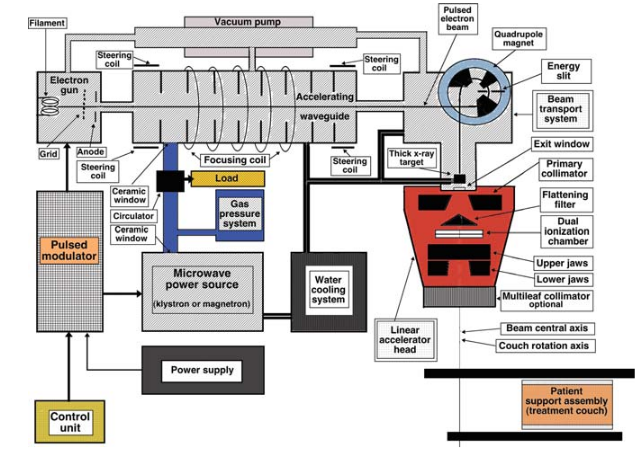
\includegraphics[width=0.9\linewidth]{images/linalc.png}
	\caption{Acelerador lineal típico usado en radioterapia \cite{podgorsak}}
	\label{fig:acelerador}
\end{figure}

\textbf{Etapa de producción de electrones}\\

La primera etapa en la generación del haz de electrones es su producción. El proceso de obtener electrones libres se realiza en lo que se denomina una \textit{arma de electrones}. En esta se obtienen electrones libres por medio de emisión termoiónica, en la que un material se calienta a altas temperaturas que le dan suficiente energía a los electrones para sobrepasar la función de trabajo del material y ser emitidos de este. Estos electrones se liberan de lo que es denominado un cátodo, y luego son acelerados, alineados y colimados, mediante un campo eléctrico que se genera con una diferencia de potencial de aproximadamente 25 keV respecto a uno o varios ánodos.\\

El material del cátodo y del cual se van a desprender electrones se elige dependiendo de las condiciones de operación de la maquina. Para aplicaciones de baja corriente, como en los tubos de rayos catódicos, se usan óxidos metálicos que se operan a 800°$C$ y a una densidad de corriente de 1 $A/cm^2$. Sin embargo, para aplicaciones donde se requiere más capacidad de producción se usan los denominados cátodos dispensivos, que son matrices de tungsteno dopado con óxidos de bario, calcio y aluminio y son operados a temperaturas de 1100°$C$.\\ 

Para tener control sobre la corriente emitida por el cátodo, se incorpora una malla de control que limita el paso de electrones del cátodo al ánodo.\\

\textbf{Etapa de generación de microondas}\\

Para acelerar los electrones producidos se usa un mecanismos de resonancia con microondas. Para generar las microondas con la suficiente intensidad es posible usar un \textit{magnetrón} o un \textit{klystron}.\\

En un magnetrón se tiene un cátodo en la mitad de una cavidad que emite electrones por efecto termoionico. Por medio de un par de imanes en la parte superior e inferior de la cavidad, y a través de una diferencia de potencial, estos electrones se dirigen en una trayectoria helicoidal a un ánodo que rodea el emisor. En el ánodo hay cavidades más pequeñas que sirven como circuito resonante, cuando un electrón pasa cerca se amplifica el campo electromagnético oscilante que este produce a su alrededor. Este efecto, combinado con un modulador de pulsos para controlar la producción de electrones en el cátodo, genera ondas en el espectro de 2856 MHz a 2998 MHz, que son recolectadas y posteriormente emitidas por una antena. Un diagrama del funcionamiento del magnetrón se encuentra en la figura \ref{fig:magnetron}.\\

\begin{figure}[H]
	\centering
	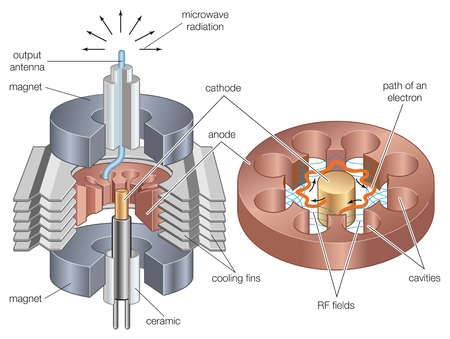
\includegraphics[width=0.7\linewidth]{images/magnetron.jpg}
	\caption{Magnetrón\cite{magne}}
	\label{fig:magnetron}
\end{figure}

El magnetrón se usa para acelerar electrones a energía menores a 20 MeV, en caso de requerirse energías mayores se debe usar un klystron. En un klystron se tiene de igual manera un cátodo que emite un haz de electrones por efecto termoiónico que son acelerados y dirigidos hacia un ánodo mediante una diferencia de potencial. Estos electrones son separados en paquetes mediante un campo electromagnético oscilante en una primera cavidad. Estos paquetes viajan a través de diversas cavidades, empujado electrones en estas a la misma frecuencia que el campo magnético de entrada. Este movimiento genera una amplificación de la radiofrecuencia de entrada que se emite en forma de microondas. Un esquema de un klystron se muestra en la figura \ref{fig:klystron}.\\

\begin{figure}[H]
	\centering
	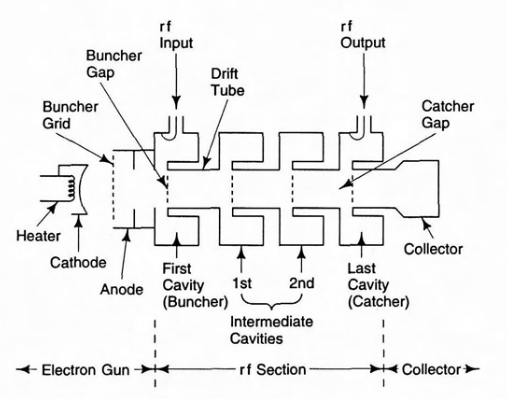
\includegraphics[width=0.7\linewidth]{images/klystron.png}
	\caption{Klystron\cite{karzmark1993medical}}
	\label{fig:klystron}
\end{figure}

\textbf{Etapa de aceleración en guía de onda y redireccionamiento}\\

Para acelerar los electrones a la energía deseada mediante la interacción con las microondas producidas en el magnetrón o en el klystron se usa el principio de onda estacionaria. \\

Inicialmente se tiene una haz de electrones colimados provenientes del arma de electrones, este haz se subdivide en paquetes de tal manera que estén distanciados media longitud de onda entre ellos. \\
 
Después, estos paquetes de electrones pasan por una guía de onda particionada en cavidades con dimensiones tales que una microonda entrante por un extremo viaje a través de esta y se refleje de tal manera que se cree una onda estacionaria.  Si el tamaño de cada cavidad de la guía de onda es el adecuado, exactamente un cuarto de la longitud de onda, entonces se tendrá  un efecto de aceleración de los paquetes de electrones puesto que se van a encontrar múltiples veces con la misma fase de la onda. Como resultado se tiene un haz de paquetes de electrones acelerados hasta cierta energía dependiente del diseño de la guía de onda.\\

Después del proceso de aceleración, los electrones pueden o no ser redireccionados 270 grados según la estructura del acelerador. Este proceso se realiza en lo que se denomina el gantry de la maquina y se realiza mediante la aplicación de un campo magnético que desvía a trayectoria de los electrones acelerados. Además de cambiar la dirección del haz, este proceso también sirve como filtro para electrones de muy alta o muy baja  energía que no son deseados en el haz, puesto que se desvían de la trayectoria de los demás electrones y son apartados del haz. Finalmente, se obtiene un haz uniforme de alta energía de electrones. \\ 

\textbf{Etapa de producción y adecuación de rayos X}\\

Para producir rayos X con mayor poder de penetración que los electrones se requiere la colisión con un objetivo de tungsteno. En este proceso, la trayectoria de los electrones es modificada por la interacción columbiana con los núcleos de los átomos del material objetivo. Este cambio de trayectoria se traduce en una aceleración sobre una partícula cargada, que en consecuencia emite cierta parte de su energía en forma de radiación electromagnética. \\

Teniendo en cuenta que los electrones pueden sufrir múltiples procesos de este estilo a lo largo de su trayectoria en el material, se tiene al final un haz de rayos X distribuido en múltiples direcciones en el espacio y además con un espectro de energía que puede alcanzar hasta la energía máxima que tenían los electrones incidentes. En la figura \ref{fig:distribucionAngular} se muestra un esquema de la distribución espacial que se obtiene después de la colisión dependiendo de la energía inicial del haz de electrones. \\

\begin{figure}[H]
	\centering
	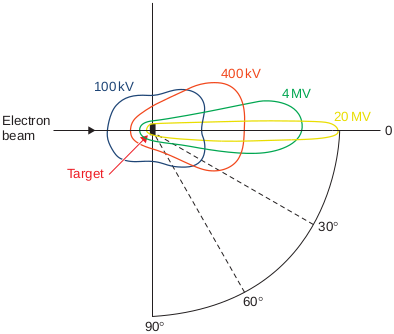
\includegraphics[width=0.7\linewidth]{images/distribucionAngular.png}
	\caption{Distribución angular de rayos X producidos por la colisión con un objetivo}
	\label{fig:distribucionAngular}
\end{figure}

Para tener control sobre la calidad geométrica del haz es necesario implementar una serie de filtros y colimadores que ajustan la forma final del haz. En la figura \ref{fig:filtrosRayosX} se muestra un esquema de los filtros usados. En este se muestra un colimador primario inmediatamente después de la producción de la radiación en el objetivo, limitando la cantidad de radiación que se dispersa en direcciones no deseadas. Después se tiene un filtro aplanador móvil, que se usa para homogeneizar espacialmente la intensidad del haz resultante y a continuación se posiciona una cámara de ionización que mide la cantidad de radiación que se ha impartido hasta el momento, para luego finalmente ser colimado por una última vez, homogeneizando más el haz resultante.\\
\begin{figure}[H]
	\centering
	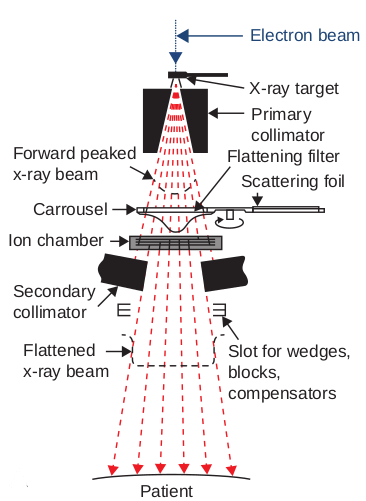
\includegraphics[width=0.7\linewidth, height=10cm]{images/filtros.png}
	\caption{Sistema de filtrado y colimado de rayos X\cite{khan2014the}}
	\label{fig:filtrosRayosX}
\end{figure}
En aplicaciones modernas se incluye un ultimo colimador denominado MLC (Multileaf Collimator) que consiste en múltiples laminas móviles de plomo que permite moldear la forma del campo final de radiación para ajustarse a geometrías convenientes en el tratamiento.\\


\textbf{Mecanismos de soporte al funcionamiento}\\

Existen sistemas auxiliares que no participan en la etapa de aceleración de electrones ni producción de rayos X, pero son cruciales para los componentes que si intervienen. Entre los principales se encuentran el sistema de refrigeración con agua, que evita el recalentamiento de los componentes por disipación de energía, así como el sistema que crea el vacío requerido para que los electrones viajen libremente sin verse alterados por moléculas de aire.\\

La maquina tiene además un sistema de frenado de radiación dispersa residual que evita que esta se libere en cantidades perjudiciales al ambiente y un sistema de alineación para ajustar la geometría del haz con respecto a la posición del paciente.\\



\subsection{Procedimientos en radioterapia}

El principal objetivo de un tratamiento con radioterapia es eliminar células cancerígenas localizadas generando la menor cantidad de daño posible a las células sanas al rededor de estas. Realizar esta tarea de manera segura y eficiente tanto para el paciente como para el personal operativo requiere de sistemas sofisticados que se han venido perfeccionando a lo largo de los años\cite{radioterapia}\cite{cancer.net_2020}.\\

Para destruir estas células de cáncer se usa radiación ionizante producida de diferentes maneras. Esta radiación puede usarse como tratamiento principal, o como apoyo a un procedimiento de cirugía o quimioterapia. El tratamiento puede usarse para eliminar por completo el cáncer, o, en los casos donde no es posible eliminarlo, reducir su extensión para minimizar síntomas y mejorar la calidad de vida del paciente.\\

Un procedimiento en radioterapia puede dejar efectos secundarios dado que no se puede eliminar solamente el tejido dañado sin eliminar parte del bueno. Algunos efectos secundarios comunes pueden ser la fatiga o problemas cutáneos, o dependiendo de la localización del cáncer, podrían haber otro tipo de efectos, como la caída del cabello, dificultad para tragar o respirar, nauseas, vomito, diarrea, incontinencia o infertilidad. Por lo general, estos síntomas son pasajeros, pero dependiendo de qué tan agresivo es el tratamiento, pueden tener consecuencias a largo plazo. Un tratamiento de radioterapia mal planeado o mal ejecutado puede traer consecuencias catastróficas, pudiendo incluso causar la muerte de un paciente.\\

La radiación usada para los tratamientos puede venir de diversas fuentes. Se denomina radioterapia interna o braquiterapia cuando la fuente de la radiación es introducido dentro del paciente cerca a su tejido dañado. Pueden ser pequeños fragmentos metálicos que contienen material radioactivo que liberan la mayor parte de la radiación en el tejido dañado, o también líquidos inyectados que cumplen la misma función. Este tipo de terapia se usa cuando el tejido es de fácil acceso, como en el caso de cáncer de próstata, cabeza o cuello.\\

Cuando el tejido enfermo no es de fácil acceso se puede usar la radioterapia de haz externo, en la cual se usa un haz de radiación ionizante producido externamente al paciente. Este haz puede ser de fotones, electrones o protones, dependiendo del tipo de patología y los recursos disponibles en el centro médico. En la sección anterior se describió un dispositivo usado para tratamientos con fotones, que son lo comúnmente encontrados en centros de radioterapia por su versatilidad para tratar diversos tipos de cáncer. La terapias con protones y electrones se usan en ciertos casos específicos, donde el tejido enfermo es fácilmente accesible, proporcionando menor daño al tejido sano circundante debido al menor poder penetrativo de estas partículas, siendo útiles, por ejemplo en casos de cáncer de piel.\\

La terapia con fotones es la más usada y desarrollada hasta el momento, por lo que existen actualmente múltiples técnicas que minimizan los riesgos asociados a los tratamientos con radiación y velan por la comodidad del tratamiento para el paciente. Dos de las técnicas más usadas son IMRT(radioterapia de intensidad modulada) y VMAT(arcoterapia volumétrica de intensidad modulada), en las cuales se administra radiación acomodada geométricamente a la forma de la lesión, administrando altas cantidades de dosis al tejido tumoral y reduciendo la dosis entregada al tejido sano. En radioterapia IMRT se administran un numero fijo de direcciones de irradiación y distribuciones producidas por el MLC de la maquina, mientras que en VMAT la radiación administrada se va ajustando a la forma del tumor conforme se varía continuamente la dirección de irradiación con la máquina. También existen procedimientos especiales como la radiocirugia, en donde se aplican haces finos de radiación desde diversos ángulos, enfocándolos a un determinado tumor.\\



La función de un físico médico consiste en diseñar el plan de tratamiento para administrar la dosis requerida por el médico de manera efectiva. Para diseñar el plan se requiere apoyo de un sistema de imágenes obtenidas por tomografía o resonancia magnética que dan información espacial tridimensional de la patología del paciente. Con esta información, el físico médico se apoya en un sistema de planeación(TPS) que permite determinar la mejor manera de suministrar la radiación procurando mantener bajo los niveles estipulados la dosis entregada al tejido sano y entregando la mayor cantidad de dosis al tejido enfermo.\\

En general, un tratamiento para entregar cierta cantidad de dosis se realiza a lo largo de un mes, en donde el paciente asiste diariamente a sesiones de entrega de dosis y monitoreo de la evolución de su estado. \\    

\section{Interacción radiación y partículas cargadas con materia}
\subsection{Interacción de fotones con materia}
Ahora, una vez determinadas las unidades con las que se medirá la radiación absorbida, es necesario establecer los mecanismos mediante los cuales esta interactúa con la materia y deposita energía en ella. Por lo tanto, a continuación se expondrán los procesos en los cuales los fotones depositan energía en los átomos y se presentará una manera de cuantificar este proceso numéricamente.  \\

Una partícula de un haz de radiación sin carga tiene alta probabilidad de pasar por una lámina delgada de algún material sin perder energía, mientras que un haz de partículas cargadas probablemente pierda parte o la totalidad de su energía. Ambos procesos hacen parte importante del proceso de transmisión de energía a la materia por parte de un haz de radiación. En esta sección estudiaremos los procesos mediante los cuales los fotones depositan energía.\\

\noindent
\textbf{Atenuación exponencial}\\


Consideremos un haz mono-energético de partículas sin carga que incide perpendicularmente en la superficie de un material de espesor $L$. Si inicialmente existen $N_0$ partículas en el haz, después de atravesar el material alguna proporción de estos habrá sido absorbida en alguna de las diversas interacciones que pueden ocurrir con las partículas cargadas en el medio. En una primera aproximación, consideramos el caso ideal en que ninguna radiación secundaria es producida, es decir, las partículas del haz o bien son absorbidas completamente, o bien pasan a través sin perder nada de su energía.\\

Para dar cuenta de este efecto de absorción general mediante diferentes mecanismos, se propone el modelo de atenuación exponencial, en el que se modela el cambio en el numero de partículas en el haz $dN$ mediante la relación
\begin{equation}
	dN=-\mu N dl,
\end{equation}  
donde $\mu$ es denominado el \textit{coeficiente de atenuación lineal} y está asociado a la probabilidad de que una partícula del haz sea absorbida en su trayecto por una distancia $dl$. Además, si esta cantidad se divide por la densidad $\rho$ del medio de atenuación, se obtiene el coeficiente másico de atenuación $\mu/\rho$.\\

Integrando esta relación entre $0$ y el espesor $L$ del material, obtenemos la relación
\begin{equation}
	N=N_0 e^{-\mu L},
\end{equation}
que es denominada la ley de atenuación exponencial, que da cuenta del número de partículas que no fueron absorbidas por el medio en su recorrido por el material de espesor $L$.\\

Para determinar este coeficiente asociado a la probabilidad de absorción, es necesario estudiar los mecanismos principales en los que se transfiere o deposita energía de un haz de partículas sin carga. En el contexto de radioterapia, existen tres principales mecanismos de transmisión de energía  de fotones a partículas con masa. A continuación se relacionan estos y una descripción de cómo modifican este coeficiente de atenuación.\\

\noindent
\textbf{Dispersión elástica e ineslástica}\\

Los procesos de dispersión se dan cuando un fotón incidente con cierta energía interactúa directamente con el átomo y no es absorbido por este. Existen dos tipos de dispersión, la primera es la dispersión elástica o de Rayleigh, en la cual el fotón es dispersado elásticamente, es decir, con un traspaso esencialmente nulo de energía al átomo, solo es redireccionado un ángulo pequeño respecto a la dirección de incidencia. Una representación de este proceso se puede ver en la figura \ref{fig:rayleigh}.\\
\begin{figure}[H]
	\centering
	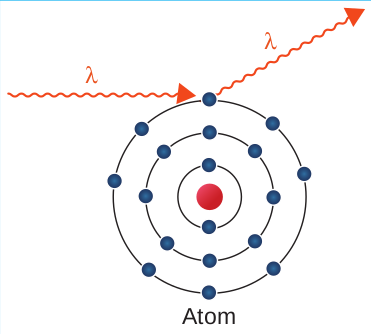
\includegraphics[width=0.7\linewidth]{images/rayleigh.png}
	\caption{Dispersión elástica\cite{khan2014the}}
	\label{fig:rayleigh}
\end{figure}
En este caso, el átomo se mueve solo lo suficiente para conservar el momento lineal. Por lo tanto, la contribución a la energía depositada por este proceso es despreciable. La contribución de este proceso al coeficiente másico de atenuación es despreciable a energías superiores a $10 keV$, que es mucho menor al rango de energía usado en radioterapia, por lo que no será tenido en cuenta.  \\

Por otro lado, el segundo tipo de dispersión es el denominado \textit{efecto Compton}. En este, un fotón incidente en un átomo interactúa de forma no elástica con un electrón, que se asume libre y estacionario, impartiendo cierta energía en él. Para que este proceso suceda, la energía de ligadura del electrón al átomo debe ser mucho menor a la energía del fotón incidente. Este proceso se ve ilustrado en la figura \ref{fig:compton}.\\
\begin{figure}[H]
	\centering
	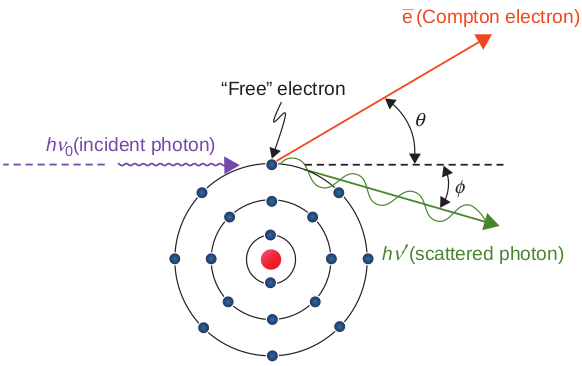
\includegraphics[width=0.7\linewidth]{images/compton.png}
	\caption{Dispersión no elástica- Efecto Compton \cite{khan2014the}}
	\label{fig:compton}
\end{figure}
En este proceso, el electrón es desligado del átomo y obtiene cierto momento en dirección $\theta$ con respecto a la dirección del fotón incidente. De la misma manera, el fotón es dispersado un ángulo $\phi$. \\

Este mecanismo puede ser estudiado desde la cinemática de la colisión de dos partículas relativistas. A partir de la conservación de energía y momento, es posible deducir las condiciones 
\begin{equation}
E=h \nu_{0} \frac{\alpha(1-\cos \phi)}{1+\alpha(1-\cos \phi)},
\end{equation}
\begin{equation}
h \nu^{\prime}=h \nu_{0}=\frac{1}{1+\alpha(1-\cos \phi)},
\end{equation}
\begin{equation}
\cot \theta=(1+\alpha) \tan \phi / 2,
\end{equation}
donde $h\nu_0$ es la energía del fotón incidente, $h\nu'$ es la energía del fotón dispersado, $E$ es la energía del electrón liberado y $\alpha=h\nu_0/m_0c^2$ con $m_0$ la masa en reposo del electrón. \\

Ahora, la probabilidad de que suceda un evento de este tipo puede calcularse mediante la sección eficaz del proceso. Esta viene dada por la fórmula de \textit{Klein-Nishina}, que expresa que la sección eficaz diferencial para este proceso es
\begin{equation}
\label{eqn:KleinNishina}
\frac{d_{e} \sigma}{d \Omega_{p}}=\frac{r_{0}^{2}}{2}\left(\frac{h \nu^{\prime}}{h \nu}\right)^{2}\left(\frac{h \nu}{h \nu^{\prime}}+\frac{h \nu^{\prime}}{h \nu}-\sin ^{2} \phi\right),
\end{equation}
donde $r_0=e^2/m_0c^2$ es el radio clásico del electrón.\\

La sección eficaz total por electrón bajo el modelo de Klein-Nishina se puede obtener integrando la ecuación \eqref{eqn:KleinNishina} sobre los posibles ángulos de dispersión del fotón, así
\begin{equation}
\begin{split}
_{e}\sigma&=2 \pi \int_{\phi=0}^{\pi} \frac{d_{e} \sigma}{d \Omega_{\phi}} \sin \phi d \phi\\
&=2 \pi r_{0}^{2}\left\{\frac{1+\alpha}{\alpha^{2}}\left[\frac{2(1+\alpha)}{1+2 \alpha}-\frac{\ln (1+2 \alpha)}{\alpha}\right]+\frac{\ln (1+2 \alpha)}{2 \alpha}-\frac{1+3 \alpha}{(1+2 \alpha)^{2}}\right\}.
\end{split}
\end{equation}
\\

Esta sección eficaz total por electrón es independiente del número atómico($Z$) del material con el que la radiación está interactuando,
\begin{equation}
	_{e}\sigma\propto Z^0,
\end{equation}
dado que no se está considerando que el electrón esté ligado al núcleo. De esta manera, la sección eficaz total por átomo con número atómico $Z$, viene dada por 
\begin{equation}
	_{a}\sigma=Z\cdot _{e}\sigma,
\end{equation}
y en consecuencia, el coeficiente de atenuación másico asociado al efecto Compton viene dado por 
\begin{equation}
	\frac{\sigma_c}{\rho}=\frac{N_{A}Z}{A}  _{e}\sigma,
\end{equation} 
donde $N_A$ es el número de Avogadro, $A$ es el peso molecular de los átomos del material y $\rho$ su densidad.\\

\textbf{Efecto Fotoeléctrico}\\

El efecto fotoeléctrico es el fenómeno en el cual un fotón incidente de radiación es absorbido por un átomo, y en consecuencia un electrón es liberado de este. En este proceso, toda la energía del fotón incidente $h\nu$ es transferida al electrón, que al final del proceso habrá adquirido una energía cinética de $T=h\nu-E_b$, donde $E_b$ es la energía de enlace del electrón al átomo. En este fenómeno es necesaria la presencia del núcleo atómico para lograr una conservación de momentos en el proceso. \\

Además del electrón liberado de la ligadura con el átomo, otros efectos secundarios pueden surgir a partir de esta interacción. Cuando el electrón es expulsado del átomo, esté deja un espacio libre que puede ocupar un electrón de una capa superior, y en este proceso de transición se producen rayos X característicos. También, esta energía liberada por la transición atómica puede ser absorbida por otro electrón en un nivel energético superior, lo que provoca que éste también sea liberado, en cuyo caso se denomina un \textit{electrón Auger}. Este proceso se ilustra en la figura \ref{fig:fotoelectrico}\\
\begin{figure}[H]
	\centering
	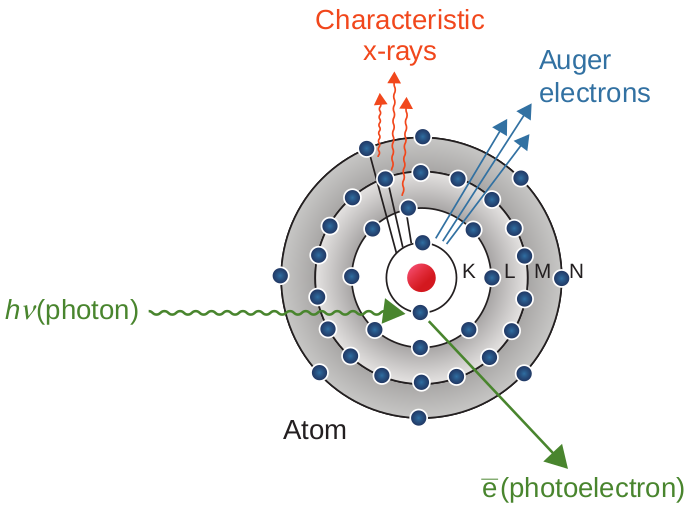
\includegraphics[width=0.7\linewidth]{images/fotoelectrico.png}
	\caption{Efecto fotoeléctrico \cite{khan2014the}}
	\label{fig:fotoelectrico}
\end{figure}

La probabilidad de que la interacción de efecto fotoeléctrico ocurra depende del numero atómico del material y de la energía del fotón incidente. Es posible describir aproximadamente su efecto sobre el coeficiente de atenuación mediante la sección eficaz por interacción
\begin{equation}
	\frac{\tau}{\rho}\propto \frac{Z^n}{E^m},
\end{equation} 
donde $Z$ es el número atómico del material, $E$ es la energía del fotón incidente, y $n$ y $m$ son números dependientes de la energía. Particularmente, $n\approx 4$ a $0.1 MeV$ aumentando gradualmente a $n\approx4.6$ a $3 MeV$ y $m\approx3$ a $0.1 MeV$ decreciendo a $m\approx1$ a $5 MeV$.\\

\textbf{Producción de pares}\\

Finalmente, si la energía de los fotones es superior a $1.02 MeV$ se puede producir interacción por producción de pares. En este proceso el fotón incidente interactúa con el campo electromagnético producido por el núcleo, produciéndose un par electrón-positrón, como se ilustra en la figura \ref{fig:Pares}. Para que este proceso suceda es necesario que el electrón tenga como mínimo la energía en reposo de dos electrones, que es de $0.511 MeV$. En este caso tenemos como ecuación de conservación de energía
\begin{equation}
	E=2m_0c^2+T^{+}+T^{-},
\end{equation}
donde $T^{+}$ es la energía del positrón y $T^{-}$ es la energía del electrón.\\

\begin{figure}[H]
	\centering
	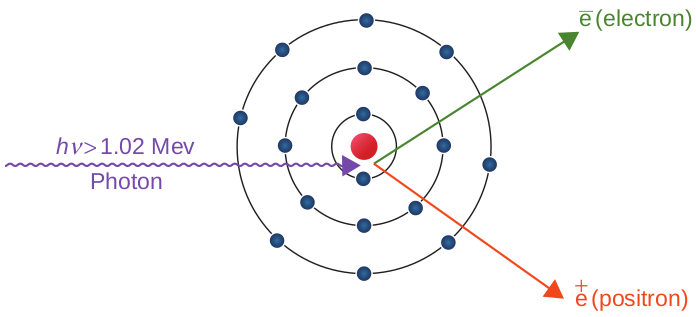
\includegraphics[width=0.7\linewidth]{images/produccionPares.png}
	\caption{Producción de pares \cite{khan2014the}}
	\label{fig:Pares}
\end{figure}

La probabilidad de que este suceso ocurra puede cuantificarse mediante la sección eficaz diferencial de Bethe y Heitler, que predice 
\begin{equation}
	d_{p}\kappa=\frac{\sigma_0 Z^2 P}{h\nu -2m_0c^2}dT^{+}, 
\end{equation}
denotando por $\sigma_0=r_{0}^2/137$ y $P$ una función de $E$ y $Z$, con lo cual la sección eficaz por átomo se calcula como
\begin{equation}
	_{p}\kappa=\sigma_0Z^2\overline{P},
\end{equation}
donde $\overline{P}$ es el promedio de la función $P$ sobre el intervalo de energía estudiado.\\

De esta manera, este proceso contribuye en el coeficiente de atenuación másico como
\begin{equation}
	\frac{\kappa}{\rho}=_{p}\kappa\frac{N_A}{A}.
\end{equation}.

Juntando todas las contribuciones por los diferentes procesos de interacción se obtiene un coeficiente de atenuación másico total $\mu/\rho$
\begin{equation}
	\frac{\mu}{\rho}=\frac{\sigma_c}{\rho}+\frac{\tau}{\rho}+\frac{\kappa}{\rho},
\end{equation}
que describe la capacidad de atenuación de determinado material ante la radiación.

En la figura \ref{fig:importanciaRelativa} se muestra la importancia relativa de estos tres efectos dependiendo del número atómico efectivo del material y la energía del haz. Aquí las curvas muestran los puntos donde los efectos colindantes tienen la misma sección eficaz.

\begin{figure}[H]
	\centering
	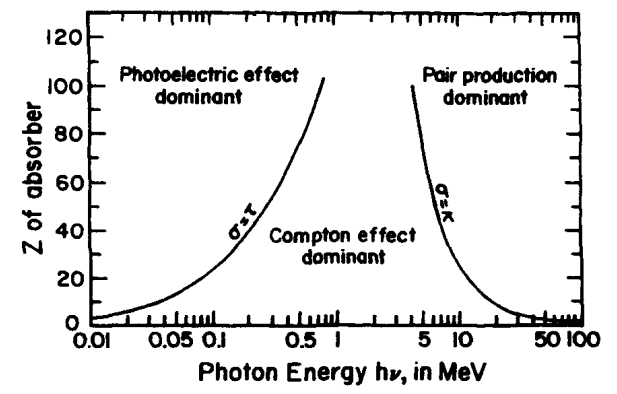
\includegraphics[width=0.7\linewidth]{images/importanciaRelativa.png}
	\caption{Importancia relativa de los tres principales tipos de interacción de fotones con la materia \cite{Attix1986}}
	\label{fig:importanciaRelativa}
\end{figure}

Así se evidencia que las interacciones más importantes de la radiación con agua en el régimen de energías de la radioterapia son las dispersiones Compton, seguidas de las contribuciones por producción de pares y finalmente, con un aporte bajo, las interacciones por efecto fotoeléctrico.  \\

\subsection{Interacción de partículas cargadas}

Las partículas cargadas, como los electrones o protones, interactúan con la materia de manera diferente a las partículas sin carga, como el fotón o neutrón. Una partícula sin carga podría pasar por la materia sin interactuar con ningún átomo y conservar toda su energía, o bien interactuar una o más veces, perdiendo su energía en el proceso. Por el contrario, una partícula cargada, al estar completamente rodeada de su campo columbiano, interactúa con cada átomo cercano a su trayectoria. Cada interacción individual transfiere una pequeña energía cinética de la partícula cargada, por lo que se puede considerar que ésta pierde energía de forma continua, en lo que es denominado la \textit{aproximación de frenado continuo}.\\

Para describir cuantitativamente el fenómeno de perdida energética continua por parte de una partícula cargada se usa la cantidad denominada \textit{poder de frenado}, $(dT/dx)_{T,Z}$, que se define como la energía promedio depositada por unidad de longitud por una partícula con energía cinética $T$ mientras se desplaza en un medio con número atómico $Z$. Si esta cantidad se divide por la densidad $\rho$ del material, se denomina el \textit{poder de frenado másico}.\\

Este poder de frenado puede separarse en dos componentes, 
\begin{equation}
	\frac{dT}{\rho dx}=\left(\frac{dT}{\rho dx}\right)_c+\left(\frac{dT}{\rho dx}\right)_r,
\end{equation}   
en donde el primer término representa perdidas de energía de la partícula por colisiones en interacciones directas de los campos de coulomb y el segundo representa perdida de energía por procesos radiativos, como el \textit{bremsstrahlung}.\\

El primer término puede ser aproximado mediante la fórmula de Bethe-Bloch, que para partículas pesadas como los protones expresa
\begin{equation}
	\left(\frac{d T}{\rho d x}\right)_{c}=2 k\left[\ln \left(\frac{2 m_{0} c^{2} \beta^{2}}{\left(1-\beta^{2}\right) I}\right)-\beta^{2} -\frac{C}{Z}\right],
\end{equation}
donde $\beta=v/c$ es el parámetro relativista de la velocidad, $I$ es el potencial de excitación medio del átomo, y $k,C$ son constantes. Y para partículas ligeras como electrones
\begin{equation}\left(\frac{d T}{\rho d x}\right)_{c}=k\left[\ln \left(\frac{\tau^{2}(\tau+2)}{2\left(I / m_{0} c^{2}\right)^{2}}\right)+F^{-}(\tau)-\delta-\frac{2 C}{Z}\right],\end{equation}
donde $\tau=T/m_0c^2$ y 
\begin{equation}F^{-}(\tau) \equiv 1-\beta^{2}+\frac{\tau^{2} / 8-(2 \tau+1) \ln 2}{(\tau+1)^{2}}.\end{equation}\\

Y finalmente, en el caso de partículas ligeras el término radiativo del poder de frenado puede ser aproximado por 
\begin{equation}\left(\frac{d T}{\rho d x}\right)_{r}=\sigma_{0} \frac{N_{A} Z^{2}}{A}\left(T+m_{0} c^{2}\right) \bar{B},\end{equation}
donde $\sigma_0=\frac{1}{137}(e^2/m_0c^2)^2$ y $\bar{B}$ es una función que varía lentamente con $Z$ y $T-$.

\section{Medidas de radiación ionizante}
Teniendo en cuenta que la radiación ionizante es particularmente peligrosa en tejidos biológicos cuando no se tiene suficiente control sobre ella, es necesario desarrollar un sistema de medida que permita describir cuantitativamente los efectos en la que un haz con cierta energía interactúa con la materia que atraviesa.\\

En primer lugar, es posible caracterizar un haz con su \textit{fluencia de partículas},denotada por $\Phi $, que se define como la cantidad diferencial dada por el cociente $dN$ por $da$, donde $dN$ es la cantidad esperada de partículas del haz que atraviesan una esfera imaginaria de sección transversal $da$.
\begin{equation}
\Phi=\frac{dN}{da}.
\end{equation}   
Con esta cantidad se puede definir la \textit{densidad de flujo}, denotada por $\phi$ como la fluencia de partículas $\Phi$ por unidad de tiempo
\begin{equation}
\phi=\frac{d\Phi}{dt}.
\end{equation}
Además, se define la \textit{fluencia de energía}, denotada por $\Psi$, como el valor esperado de energía de todas las partículas del haz que atraviesan una esfera imaginaria de sección transversal $da$.
\begin{equation}
\Psi=\frac{dE}{da},
\end{equation}
y con esta se define la densidad de flujo de energía, denotada como $\psi$, como la fluencia de energía por unidad de tiempo
\begin{equation}
\psi=\frac{d\Psi}{dt}.
\end{equation}
Por otro lado, es posible establecer unidades de medida para cuantificar la interacción de un haz con la materia. Las principales unidades de medida se presentan a continuación\\

\noindent
\textbf{Kerma($K$)}\\

Se define como la cantidad de energía cinética inicial de las partículas cargadas (electrones o positrones) que son liberadas por partículas sin carga (fotones) por unidad de masa
\begin{equation}
K=\frac{dE_{tr}}{dm},
\end{equation}
el kerma tiene unidades de $J/Kg$, denominada también Gray (Gy), ($1J/kg=1Gy$).


En un material el kerma puede ser separado en dos componentes, el kerma de colisión $K_c$  asociado a las interacciones columbianas con los electrones del material que disipan energía y el kerma radiativo $K_r$, asociado a perdidas de energía por procesos de radiación de frenado. Teniendo finalmente 
\begin{equation}
	K=K_c+K_r.
\end{equation}\\

En el caso de un haz de fotones, es posible relacionar el kerma de colisión con la fluencia de energía mediante el \textit{coeficiente másico de transferencia de energía}, denotado por $(\mu_{tr}/\rho)_{E,Z}$, que es característico para cada material y la energía del haz, así
\begin{equation}
K_c=\Psi \left(\frac{\mu_{tr}}{\rho}\right)_{E,Z},
\end{equation} 
donde $\mu_{tr}$ es el \textit{coeficiente lineal de transferencia de energía}, con unidades $m^{-1}$ y $\rho$ es la densidad del material.\\

\noindent
\textbf{Dosis Absorbida($D$)}\\

Definimos la \textit{energía impartida}($\epsilon$) por radiación ionizante en un volumen finito $V$ que contiene una masa $m$ como
\begin{equation}
	\epsilon =R_{in}-R_{out}+\sum Q,
\end{equation}
donde $R_{in}$ es la energía de las partículas con carga y sin carga que entran en el volumen $V$, $R_{out}$ es la energía de estas mismas partículas que dejan el mismo volumen, y $\sum Q$ cuenta por la energía de las partículas en reposo en $V$.\\

De esta manera, la \textit{dosis absorbida}($D$) se define como el valor esperado de energía impartida en cierto material por unidad de masa
\begin{equation}
D=\frac{d\epsilon}{dm},
\end{equation}
la cual también tiene unidades de Gray(Gy).\\

\noindent
\textbf{Dosis equivalente($H$)}\\

La \textit{dosis equivalente}($H$) se usa para incluir en la mediada los efectos que tiene la radiación sobre cierto tipo específico de tejido, mediante la inclusión de un factor de calidad $Q$
\begin{equation}
H=Q\cdot D
\end{equation},
esta tiene unidades de Sievert(Sv), que tiene las mismas unidades dimensionales que el Gray.\\

\noindent
\textbf{Exposición($X$)}\\

La \textit{exposición}($X$) se define como el valor absoluto de la carga de un signo producida cuando todos los electrones liberados por fotones en procesos de ionización son detenidos completamente en aire por unidad de masa
\begin{equation}
X=\frac{dQ}{dm},
\end{equation}
y tiene unidades de $C/kg$.
\section{Principios de dosimetría}
El objetivo principal de la dosimetría es determinar la cantidad de dosis absorbida por cierto material de manera precisa, de tal manera que sea útil para cuantificar procesos de radioterapia.
\subsection{Equilibrio de partículas cargadas}
En general, dado el alto nivel de abstracción requerido para definir cantidades como el kerma y la dosis absorbida, no es posible medirlas directamente en ninguna circunstancia, por lo que es necesario medir cantidades indirectas y relacionarlas con las deseadas. En la práctica es posible medir directamente cargas acumuladas en un electrodo, pero no energía absorbida por determinada sección de material. Por lo tanto, es común en dosimetría realizar una medida de exposición($X$) y relacionarla de cierta manera con la dosis absorbida en el medio($D$).\\

Para realizar la conversión de información de exposición a dosis absorbida es necesario la presencia de la condición de \textit{equilibrio de partículas cargadas}(CPE, charged particle equilibrium). Esta condición existe en un volumen $V$ cuando cada partícula cargada de cierto tipo y energía que deja este volumen es reemplazada por una partícula del mismo tipo con la misma energía.  Esto se cumple para un haz de radiación ionizante externo que atraviesa un materia cuya composición atómica y densidad es homogénea y no existen campos eléctricos y magnéticos incompatibles con la geometría del volumen.\\

Es posible mostrar \cite{Attix1986} que bajo esta condición y las definiciones de dosis absorbida y kerma se cumple que, para un volumen fijo 
\begin{equation}
	D=K_c=\Psi \frac{\mu }{\rho},
\end{equation}
es decir, en condiciones de equilibrio de partículas cargadas, la dosis absorbida en un punto es igual que el kerma de colisión en dicho punto.\\

Más aún, si por dos medios A y B atraviesa la misma fluencia de energía $\Psi$, entonces en condiciones de equilibrio de partículas cargadas se tiene que 
\begin{equation}
	\frac{D_A}{D_B}=\frac{(K_c)_A}{(K_c)_B}=\frac{(\mu/\rho)_A}{(\mu/\rho)_B},
\end{equation}
donde $D_{A,B}$ es la dosis absorbida en cada medio, $(K_c)_{A,B}$ es el kerma de colisión en cada medio y $(\mu/\rho)_{A,B}$ son sus coeficientes de absorción de energía.\\

Finalmente, la cantidad más fácil de medir en la práctica es la exposición, que en condiciones de equilibrio de partículas cargadas se puede relacionar con las dosis absorbida en aire mediante la ecuación
\begin{equation}
\label{eqn:ExpoDosis}
	D_{aire}=(K_c)_{aire}=X\cdot \left(\frac{W}{e}\right)_{aire},
\end{equation}
en donde $X$ es la exposición medida y  $\frac{W}{e}$ es la energía de radiación ionizante requerida para extraer una carga $e$ en aire.\\

Existen múltiples situaciones en las que se puede romper este equilibrio y que deben ser evitadas para poder usar estas relaciones. Por ejemplo, se debe evitar realizar mediciones cerca a la fuente de radiación, puesto que en esta región el campo es menos uniforme. De la misma manera, no se tiene equilibrio cerca a fronteras de inhomegeneidad en medios, como las que ocurren en un cambio de material. Igualmente, el equilibrio de partículas cargadas es más difícil de alcanzar en haces de alta energía(>10 MeV), para los cuales hay técnicas menos restrictivas para obtener relaciones como las anteriormente mencionadas.  
\subsection{Cámaras de ionización}
Si se tiene el objetivo de medir la dosis absorbida en cierto punto de un material se puede recurrir a la medición directa de cantidades como la exposición. Modernamente existen dispositivos especialmente diseñados con este objetivo y protocolos estandarizados que hacen que garantizan la precisión de las mediciones. \\

La cámara de ionización es el dispositivo más usado para realizar dosimetría con la precisión que se requiere en radioterapia. Estas existen en el mercado bajo diferentes modelos útiles en variadas condiciones de energía y calidad de haz.\\

El modelo fundamental usado para dosimetría absoluta en los laboratorios primarios es el modelo libre de aire. Un esquema de este modelo se representa en la figura  \ref{fig:freeAir}. En estas un haz de rayos X pasa por el diafragma D y pasa por el medio de dos platos paralelos entre los cuales existe una diferencia de tensión. Esta diferencia de tensión sirve para recolectar los iones generados por la ionización de aire entre los platos producida por la radiación ionizante. Además se tienen platos guardas para asegurar la uniformidad del campo eléctrico generado.\\
\begin{figure}[H]
	\centering
	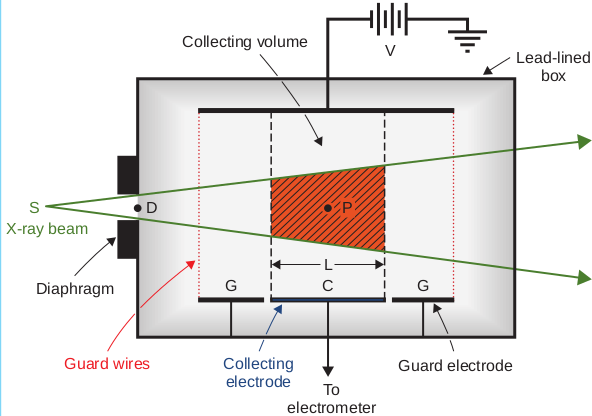
\includegraphics[width=0.7\linewidth]{images/freeAirChamber.png}
	\caption{Cámara de ionización libre de aire\cite{khan2014the}}
	\label{fig:freeAir}
\end{figure}

La carga colectada ($\Delta Q$) en los platos se puede medir precisamente mediante un electrómetro. Con esta medida se puede calcular la exposición en el punto P mediante la formula \\
 \begin{equation}
X=\frac{\Delta Q}{\rho \cdot A_{p}\cdot L}.
\end{equation}
donde $\rho$ es la densidad del aire dentro de la cámara, $A_{p}$ es el área de la sección transversal del haz en el punto P y L es la longitud del volumen de colección. Así, se tiene una medida de exposición que se puede relacionar con la dosis absorbida en el punto P mediante la formula \eqref{eqn:ExpoDosis}.

Este diseño de cámara es difícil de mantener en operación de tal manera que se obtengan siempre medidas precisas, puesto que se requieren mantener condiciones muy especificas para su funcionamiento, por lo tanto su uso está confinado a laboratorios estandarizados especializados.\\
 
En la practica en centros médicos comunes se deben usar otro tipo de cámaras calibradas respecto a las proporcionadas por estos laboratorios. En particular, el tipo más común es la cámara dedal, cuya estructura se presenta en la figura \ref{fig:farmer}.\\

\begin{figure}[H]
	\centering
	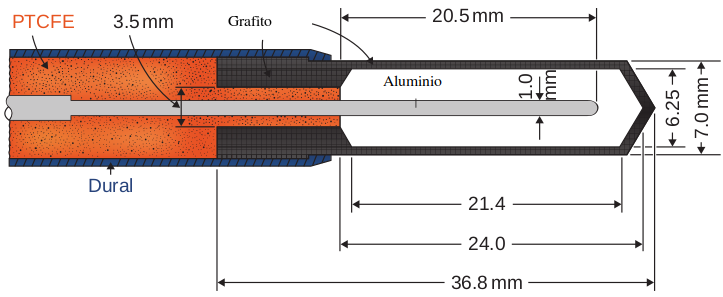
\includegraphics[width=0.7\linewidth]{images/camaraIoni.png}
	\caption{Cámara de ionización farmer\cite{khan2014the}}
	\label{fig:farmer}
\end{figure}

Su funcionamiento es similar a la cámara de aire libre. Se tiene un filamento de aluminio en el centro y una cubierta de grafito entre los cuales existe una diferencia de potencial que recolecta los iones producidos por la ionización del aire al paso de un haz de radiación ionizante. la carga colectada entre ambos electrodos se puede medir con un electrómetro y obtener una medida de dosis absorbida en consecuencia. La estructura irregular de esta  cámara hace que el campo eléctrico adentro sea inhomogeneo, por lo tanto no hay una forma absoluta de la exposición, para lo que se recurre a un factor de calibración obtenido con cámaras de aire libres.\\

Para obtener medidas fiables con este tipo de cámara se deben realizar correcciones que tengan en cuenta factores ambientales que afecten el proceso de colección de carga. Para este propósito existe el protocolo TRS 398 que permite estimar factores de corrección a las medidas para obtener una medida final fiable.\\

Este protocolo permite estimar la dosis absorbida en agua midiendo diversas cantidades ambientales con la calibrada. Para obtener una medida de dosis absorbida se debe tener una medida corregida por factores de influencia de la carga colectada $M_{Q}$, un factor de calibración $N_{D_{w},Q_{0}}$ que es proporcionado por un laboratorio de calibración para la cámara usada y relaciona la carga colectada en la cámara con la dosis absorbida en esta bajo un haz de calidad $Q_0$ usado en el laboratorio de calibración, y un factor $k_{Q,Q_{0}}$ que relaciona la calidad del haz de calibración con la calidad del haz del usuario. Con estas cantidades se calcula la dosis absorbida en agua en el haz de calidad Q como
\begin{equation}
D_{w,Q}=M_{Q}\cdot N_{D,w,Q_{0}}\cdot k_{Q,Q_{0}}.
\end{equation}

El factor $M_{Q}$ es la medida de carga colectada en la cámara obtenida con el electrómetro, corregida con factores asociados a  magnitudes de influencia que se alteran la medida de esta cantidad.\\

El primer factor esta asociado a las condiciones ambientales de presión, temperatura y humedad y que alteran la densidad del aire al interior de la cámara, por lo que alteran su capacidad de ionización. El factor de corrección asociado a esta magnitud se calcula como 
\begin{equation}
	k_{TP}=\frac{273.2+T}{273.2+T_0}\frac{P_0}{P},
\end{equation}
donde $P0,T0$ son la presión y temperatura en las condiciones de referencia, generalmente 101.3 kPa y 20 °C, y $P,T$ son la presión y temperatura en la cavidad de la cámara. Si el factor de calibración proporcionado por el laboratorio viene corregido por humedad no es necesario realizar ninguna corrección adicional, si en cambio viene reportado en aire seco se recomienda aplicar el factor $k_{h}=0.997$.\\

Por otro lado, también se tiene en cuenta el efecto de la diferencia en la medida que causa la polaridad de la cámara. Al no poseer un campo eléctrico uniforme, la cámara responde diferente dependiendo de en qué electrodo se recolecten las cargas. Para evitar este efecto la cámara se debería utilizar en la misma polarización con la que fue obtenido el factor de calibración en el laboratorio. En caso de usarse diferente o no conocerse este efecto se corrige aplicando el factor
\begin{equation}
	k_{p}=\frac{|M_{+}|+|M_{-}|}{2M},
\end{equation}
donde $M_{\pm}$ son las medidas de carga obtenidas con polaridad positiva y negativa, y $M$ es la carga medida en la polaridad que se esté utilizando.\\

Análogamente, se corrige el efecto de recombinación de iones, en el cual lo electrones liberados en el aire pueden volver a combinarse con iones producidos en el mismo proceso, reduciendo la cantidad de carga colectada en el electrómetro que se produjo por ionización. Para este proceso existe el factor de corrección
\begin{equation}
	k_s=a_0+a_1\left(\frac{M_1}{M_2}\right)++a_2\left(\frac{M_1}{M_2}\right)^2,
\end{equation}  
donde $M_1,M_2$ son medidas de carga colectada a voltajes de operación de la cámara  $V_1,V_2$ medidas en las mismas condiciones de irradiación y $a_0,a_1,a_2$ son parámetros dependientes del cociente $V_1/V_2$ que pueden ser consultados en \cite{TPR398}.\\

Finalmente, también existe un factor de corrección por el funcionamiento del electrómetro que se obtiene cuando se este se calibra independientemente de la cámara. De esta manera, la cantidad $M_Q=M_{elctrometro}\cdot \prod k_i$.\\

El factor $N_{D,w,Q_{0}}$ es el factor de calibración proporcionado por el laboratorio de calibración que se obtiene midiendo con la cámara una dosis conocida mediante otros procedimientos de dosimetría absoluta bajo un haz de calidad estándar. Por lo general, este proceso para obtener factores de calibración se debe realizar periódicamente, aproximadamente cada 2 años.\\

Finalmente,para estimar el factor $k_{Q,Q_{0}}$ se usa el $TPR_{20,10}$, que es la razón entre la dosis medida a 20 cm de profundidad en agua entre la dosis medida a 10 cm de profundidad en agua en condiciones de referencia, es decir a 100 cm de la fuente y en un campo de 10x10 cm. En la figura se muestra un esquema del montaje usado para esta medición.\\
 \begin{figure}[H]
 	\centering
 	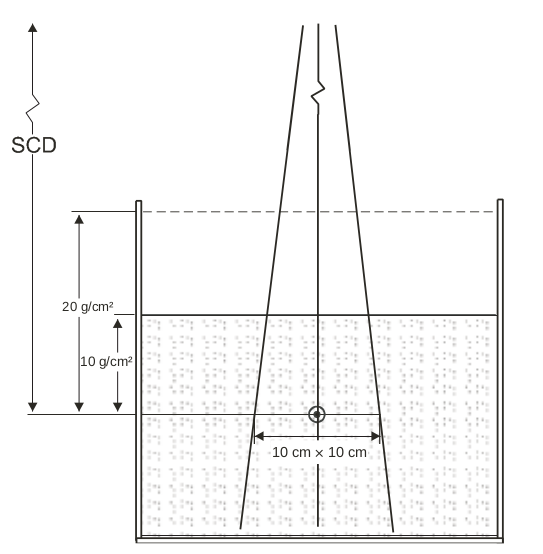
\includegraphics[width=0.7\linewidth]{images/TPR2010.png}
 	\caption{Montaje $TPR_{20,10} $ en condiciones estándar\cite{TPR398}}
 	\label{fig:TPR2010}
 \end{figure}
Una vez obtenido este factor $TPR_{20,10}$, el $k_{Q,Q_{0}}$ se encuentra tabulado dependiendo de este y del modelo de la cámara usado\cite{TPR398}.\\

Usando este protocolo de manera correcta se obtienen mediadas precisas de dosis absorbida en agua útiles para realizar calibraciones de los equipos usados en radioterapia y asegurar la calidad de los tratamientos.\\


Los aceleradores lineales usados en radioterapia traen incluida una cámara de ionización que permite determinar la cantidad de dosis entregada a un paciente después de un procedimiento. El sistema expresa esta dosis en unidades monitor (UM), de las cuales se reportan 100 UM cuando se entrega una dosis de 1Gy en un fantoma de agua a 100 cm de la fuente en un campo de 10x10 cm en el isocentro de la maquina.

\subsection{Dosimetría con películas}
Si bien con dispositivos como cámaras de ionización son precisos y útiles para medir dosis absorbidas, estas no son capaces de proporcionar un mapa de intensidad de dosis en alguna región, puesto que solo realizan mediadas puntuales. Sería inconveniente tener que medir dosis punto a punto para obtener un mapa de dosis, puesto que sería un proceso lento y suceptible a errores, y no proporcionaría una resolución en el mapa útil para propósitos en dosimetría general. \\

Este tipo de mapas de dosis determinados experimentalmente se requieren, por ejemplo, cuando se quiere realizar una comprobación de distribuciones espaciales de dosis entregadas a un paciente en un procedimiento de radioterapia.\\

Con el objetivo de poder obtener este tipo de información se ha usado la dosimetría con películas. Este tipo de dosimetría consiste en relacionar la apariencia de una película que cambia su color dependiendo de la dosis que absorba. De tal manera, se obtiene un mapa de dosis permanente de alta resolución de una manera sencilla y precisa.\\

En sus inicios, la dosimetría con películas usaba laminas fotográficas, que mediante un proceso de deposición de plata producido por la interacción con la radiación y después de un complicado proceso de revelado producía una película con información de la distribución de la dosis absorbida en ella. Este proceso ha evolucionado de diversas maneras, hoy en día su principio activo de coloración ha cambio y se denominan películas radiocrómicas, cuyo uso será estudiado en este trabajo.\\

 
\section{Películas radiocrómicas}
Como fue mencionado anteriormente, la verificación de calidad de los tratamientos de radioterapia es de gran importancia para asegurar su efectividad. Es necesario comprobar que las distribuciones de dosis que se planean correspondan suficientemente con las distribuciones que recibe el paciente. Uno de los métodos más usados actualmente para realizar esta verificación sobre mapas de dosis en dos dimensiones es el uso de películas radiocrómicas.\\

Cuando las películas radiocrómicas son sometidas a radiación ionizante, estas sufren un cambio de color debido a un proceso químico de polimerización, adquiriendo una tonalidad diferente a la que tenían sin irradiar. El cambio de color que se produce es dependiente directamente de la dosis que se absorbe en cada punto. \\

Es posible medir este cambio de tonalidad de color de diferentes maneras, por ejemplo, midiendo con un escáner la intensidad de la luz que puede atravesarla. Con esta información de cambio de tonalidad y conociendo las dosis a las que fue sometida la película, es posible establecer una correlación que permita determinar la dosis absorbida en agua en otras circunstancias midiendo únicamente el cambio de coloración. \\

Uno de los primeros procesos radiocrómicos observados fue en 1826, cuando Joseph Niepce logró capturar la imagen de una ventana luego de dejar un papel cubierto con una solución fotosensible por un periodo de 8 horas, que dejó impregnada una imagen por medio de una polimerización de carbonos insaturados producidas por la absorción de energía del haz de luz.\\

El uso y desarrollo de estas sustancias fotosensibles fue evolucionando gradualmente. Por ejemplo, en 1965 McLauglin et al \cite{McLaughlin1965} reportaron el desarrollo de una solución de derivados de trifenilmetano que producía tintes por un proceso de radiosíntesis. Avances posteriores en materiales radiocrómicos estuvieron liderados por el NIST (National Institute of Standards and Technology), y en sus versiones más tempranas eran útiles en rangos de dosis entre $10^3$ y $10^6$ Gy, por lo que su espectro de aplicación se limitaba a procesos industriales\cite{Williams2011}.\\

La transición al uso de sustancias radiocrómicas en aplicaciones no industriales se dio con la aparición de las primeras películas GAFchromic producidas por ISP Technology en 1986. Estás nuevas películas tenían una composición nueva que permitia tener transformaciones cromáticas al exponerse a dosis de apenas 5 Gy\cite{Williams2011}.\\


Desde entonces, a partir de la variación en la composición de la sustancia radiocrómica y su empaquetado, se han han venido refinando los modelos de películas disponibles. En la actualidad existen diversos tipos de películas radiocrómicas que son útiles en dosimetría en varios rangos de dosis y para diferentes propósitos. Se usan comúnmente para dosimetría relativa, teniendo un patrón de dosimetría absoluta obtenido por otro método, como medidas con cámaras de ionización. En el cuadro \ref{tab:Modelos} se muestran diferentes modelos de películas y los rangos de dosis en los que se pueden usar.\\
\begin{table}[h!]
	\centering
	\begin{tabular}{|c|c|}
		
		\hline 
		Modelo & Rango de dosis \\ 
		\hline 
		HD-V2 & 10-100Gy \\ 
		\hline 
		MD-V3 & 1-100Gy \\ 
		\hline 
		EBT-XD & 0.04-40Gy \\ 
		\hline 
		EBT2 & 0.01-30Gy \\ 
		\hline 
		EBT3 & 0.01-30Gy \\ 
		\hline 
		XR-QA2 & 0.1-20 mGy \\ 
		\hline 
	\end{tabular} 
\caption{Modelos de películas radiocrómicas}
\label{tab:Modelos}
\end{table}

En general, los modelos difieren en la estructura y composición de la película, lo que permite mejores propiedades de sensibilidad a la radiación en cierto rango o estabilidad y uniformidad en el proceso de lectura. Por lo general, la películas consisten de una capa activa que contiene la sustancia radiocrómica y sus respectivos aditivos, encapsulada en capas de poliéster que las soportan y protegen del exterior. La estructura de diversos modelos se presenta en la figura \ref{fig:Estructuras}. Las placas más usadas en el contexto de verificación de radioterapia son las de la linea EBT.\\
\begin{figure}[H]
	\centering
	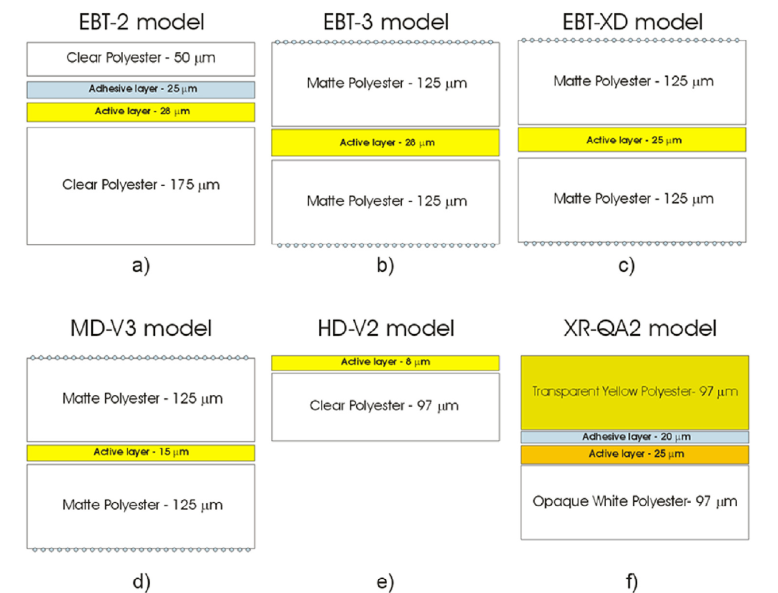
\includegraphics[width=\linewidth]{images/modelos.png}
	\caption{Estructuras de películas radiocrómicas de diferentes modelos. Tomada de \cite{Devic2016}}
	\label{fig:Estructuras}
\end{figure}

La capa activa está compuesta generalmente de cristales de poliacetilenos\cite{Williams2011}, particularmente de diacetelinos($C_4H_2$), que tras la exposición a la radiación o altas temperaturas sufren un proceso de polimerización que, junto con los aditivos, le proporciona un color diferente a la película. Específicamente, el componente activo de las películas EBT es la sal de litio del ácido pentacosa-10,12-diyonic, que sufre una 1,4-polimerización de estado solido de primer orden como se evidencia en la figura \ref{fig:reaccion}.\\  

\begin{figure}[H]
	\centering
	\subfloat[Monomeros de diacetileno\cite{Beni2017}]{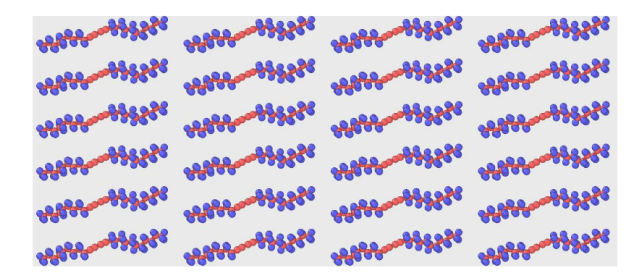
\includegraphics[width=0.5\textwidth]{images/diacetileno.png}\label{fig:diacetileno}}
	\hfill
	\subfloat[Reacción de polimerización\cite{Williams2011}]{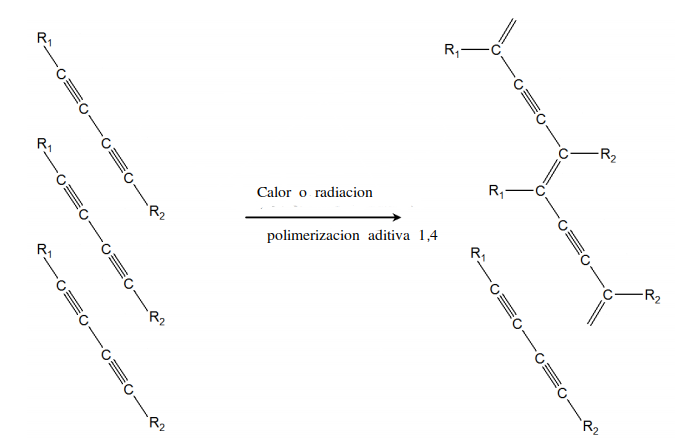
\includegraphics[width=0.5\textwidth]{images/reaccion.png}\label{fig:reaccion}}
	\caption{Polimerización de diacetilenos}
\end{figure}

El mayor cambio en coloración se produce casi instantáneamente después de la irradiación, sin embargo, la reacción puede tomar mucho más tiempo en completarse, estableciendo un tiempo de aproximadamente 24 horas para culminar este proceso \cite{Williams2011}. La velocidad de la reacción también depende de las condiciones de humedad\cite{LenMarroqun2018}, temperatura \cite{Rink2008} y exposición previa a las que está sometida la película\cite{NiroomandRad1998}. Por otro lado, estos cambios en la absorbancia de la película han sido mitigados en gran medida mediante aditivos en el componente activo, por lo que hoy en día con las modernas películas EBT3 las variaciones por estos factores resultan controlables siguiendo un protocolo sencillo de reproducibilidad. \\

También se han realizado estudios sobre la dependencia de la energía del haz en el proceso de coloración, encontrando que actualmente para las películas EBT3 la dependencia energética para energías mayores a 400 keV es mínima en un amplio rango de dosis absorbida\cite{Chemiski2010} . Además, para este tipo de placas se reporta un número atómico efectivo de $Z_{eff}=6.73$, que es muy cercano al número atómico efectivo del agua de $Z_{eff}=7.42$, por lo que la radiación interactúa de manera muy similar con ambos materiales. Lo anterior hace posible que las películas puedan ser usadas para medir dosis absorbida en agua sin factores de conversión adicionales.\\

Los cambios de absorbancia de una película cuando es sometida a la radiación pueden evidenciarse en una figura como la \ref{fig:AsorbanciaEBT3}, donde se muestra el espectro de absorción en el rango visible de una película EBT3 antes y después de ser irradiada con 5 Gy.\\
\begin{figure}[H]
	\centering
	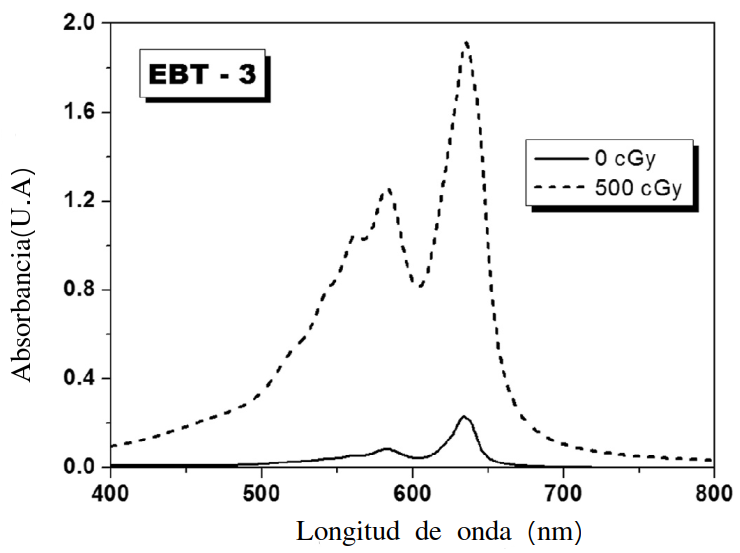
\includegraphics[width=0.7\linewidth]{images/absorbancia.png}
	\caption{Espectro de absorción de película EBT3. Tomada de \cite{Devic2016}}
	\label{fig:AsorbanciaEBT3}
\end{figure}

En esta se evidencia que la región del espectro donde se produce el mayor cambio de absorbancia es a rededor de 633 nm, en la región roja del espectro.\\

Para medir de manera práctica la absorbancia de una película irradiada existen diversos métodos. El más común es usar un escáner óptico, que proporciona una medida de la intensidad de la luz que la atraviesa. Un esquema de funcionamiento de un escáner común se muestra en la figura \ref{fig:escaner}.\\ 
\begin{figure}[H]
	\centering
	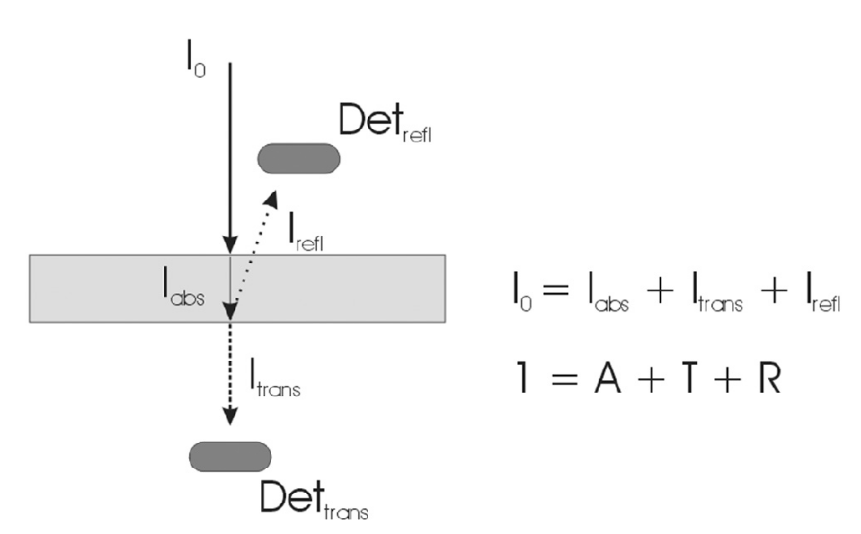
\includegraphics[width=0.7\linewidth]{images/escaner.png}
	\caption{Esquema de funcionamiento de escáner. Tomada de \cite{Devic2016}}
	\label{fig:escaner}
\end{figure}

El escáner proporciona una medida de cuánta luz deja pasar la película en cierto intervalo del espectro. Por ejemplo, en un escáner de transmitancia común  se proporciona información de cuánta intensidad transmitida $I_{tr}$ atravesó la película una intensidad inicial $I_0$. La forma más común en la que se almacena esta información en las aplicaciones consideradas es mediante una matriz RGB(red, green, blue) de 16 bits por canal. \\

Es decir, se almacena como 3 capas, cada una con información de una región del espectro analizado, el verde , el rojo o el azul, y cada pixel en cada capa adquiere un valor entre $0$ y $2^{16}-1$, que representa qué tanta intensidad de luz en el espectro fue medida en la posición del pixel. Concretamente, la información que proporciona la película resulta en tres matrices, una por cada color, que en cada entrada tiene un valor numérico que representa la cantidad de luz que se midió en la posición del pixel. Además, cada matriz RGB que reprensenta una imagen escaneada tiene una resolución expresada en ppi(pixels per inch), que especifica cuantos pixeles en la imagen adquirida hay en una pulgada del obejto escaneado en el mundo real.\\

Con esta información es posible construir la \textit{transmitancia}$(T)$ en cada color de cada pixel, que se define como 
\begin{equation}
	T=\frac{I_{tr}}{I_0}=\frac{VP}{2^{16}-1},
\end{equation}
donde $VP$ es el valor del pixel medido por el escáner. Y con esta con esta se define la \textit{densidad óptica} $DO$ como 
\begin{equation}
	DO=-\log_{10}(T)=\log \frac{2^{16}-1}{VP}.
\end{equation}\\

Estos valores caracterizan los cambios de color de la película ante radiación medidos por un escáner, y serán útiles para establecer calibraciones que permitirán determinar planos de dosis.\\

En el proceso de escaneo existen varias variables que pueden modificar la transmitancia medida en cada pixel. Por ejemplo, se han reportado diferencias en las medidas de transmitancia dependiendo de la orientación de la película en el escáner\cite{mayers}. Este efecto es debido a que la luz del escáner es polarizada en una dirección y la película irradiada actúa como un polarizador que modifica la intensidad transmitida dependiendo de la orientación con respecto a la dirección de polarización.\\

Otra circunstancia que afecta la medida es la posición de la película en el escáner. Existe un efecto óptico en el sistema que provoca un aumento de la sensibilidad en el escáner cerca a los bordes laterales de este, que puede provocar una medida de más coloración, sobreestimando la dosis que recibió la película en esa región.\\

También se reportan cambios en la medida cuando la película se somete a cierto estrés mecánico\cite{Yu2006}, por ejemplo en el área de corte, dado que se altera la estructura y dimensiones de las capas que conforman la película. En tal caso, el efecto sobre la transmitancia medida es irregular, por lo que no se puede determinar precisamente cómo cambió la coloración cerca al corte.\\

Finalmente, también pueden existir defectos en la superficie de escaneo, como partículas de polvo o rayaduras, así como pixeles específicos del sensor del escáner que estén dañados. Todos estos factores influyen de alguna manera en la correlación final que se hace para obtener mapas de dosis. En caso de que su influencia sea importante, se deben aplicar ciertas correcciones en el procedimiento para obtener resultados adecuados.\\

Para obtener información de dosis a partir de la transmitancia medida en una película es necesario realizar un procedimiento de calibración. Este consiste en asociar las medidas de transmitancia en determinado canal de la película escaneada con las dosis que iniciaron el proceso de coloración que fueron medidas con otro mecanismo, por ejemplo, una cámara de ionización. La figura \ref{fig:EbtSin} muestra una película EBT2 sin irradiar y la figura \ref{fig:EbtCali} muestra la película irradiada con $11.1 ,  19.8, 22.9, 27.6, 37.1, 74.9, 102.4, 129.6, 151.9$ y $222.6 $ cGy.\\

\begin{figure}[H]
	\centering
	\subfloat[Película EBT2 sin irradiar]{
\includegraphics[width=0.5\textwidth]{images/fondoblancoLandscape-1.png}\label{fig:EbtSin}}
	\hfill
	\subfloat[Película EBT2 irradiada]{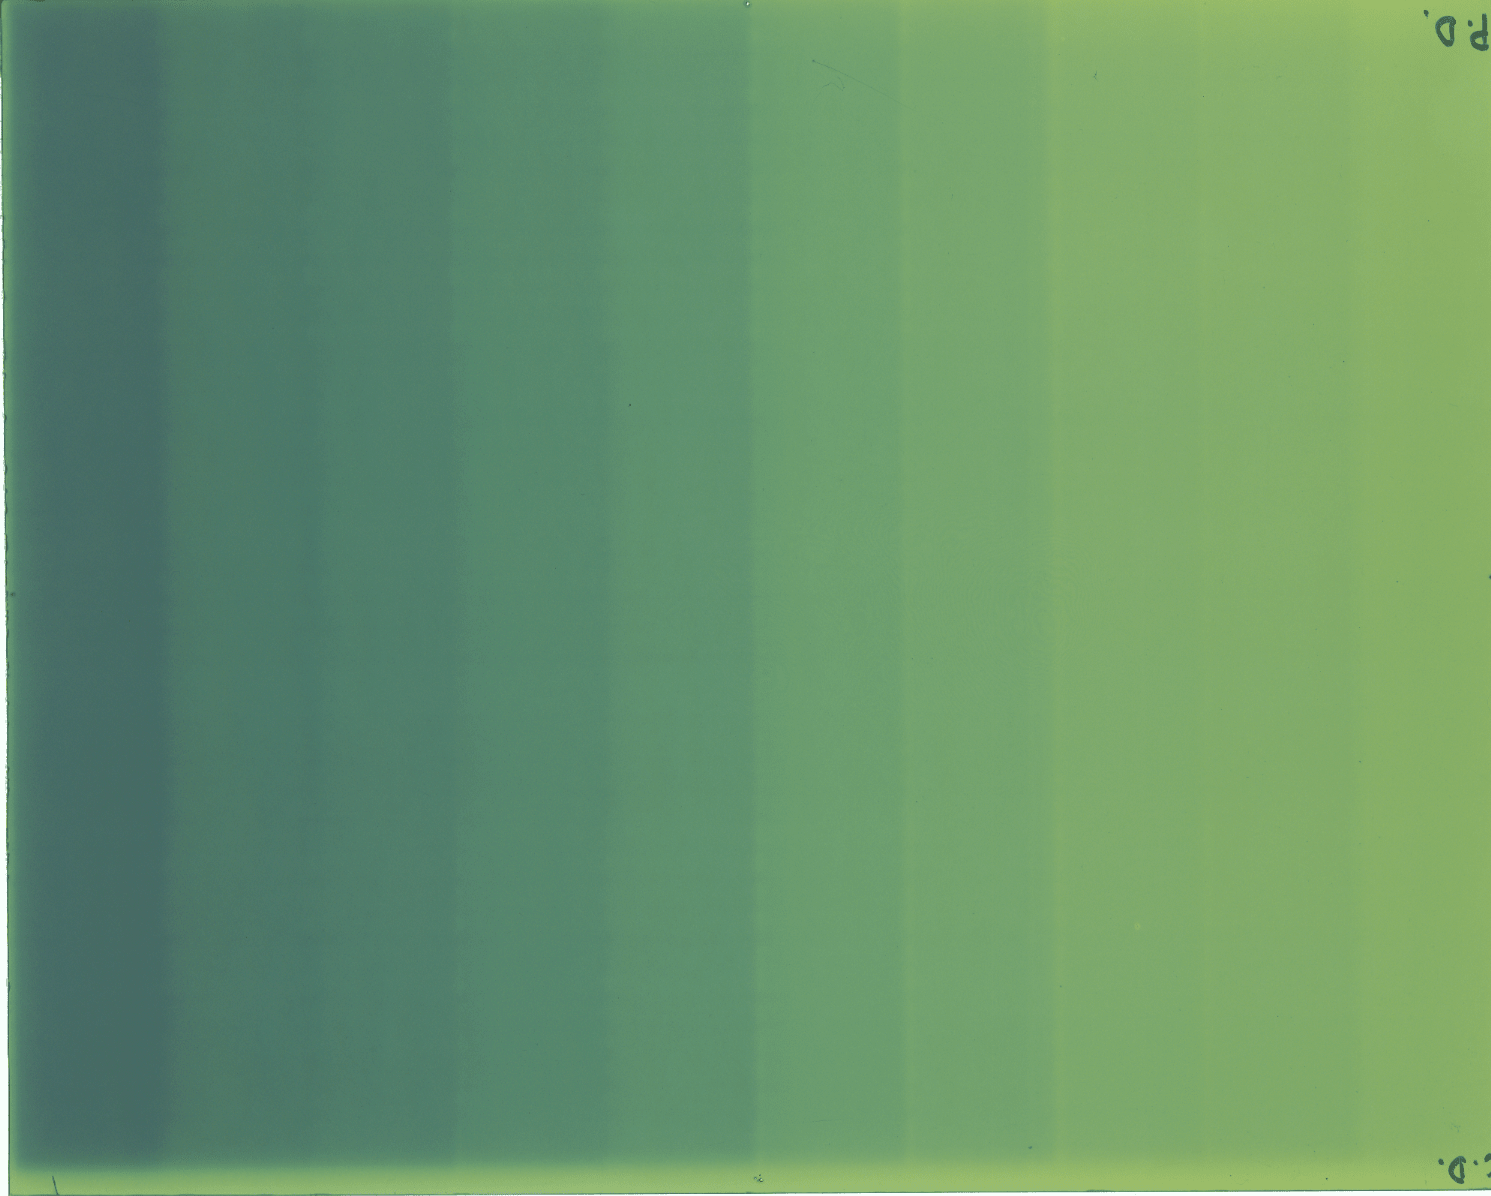
\includegraphics[width=0.5\textwidth]{images/calibracionSimpleLandscape.png}\label{fig:EbtCali}}
	\caption{Película EBT2 antes y después de irradiación}
\end{figure}

Promediando el valor de las transmitancias en cada canal de color en un región de interes(ROI) en cada una de las franjas, es posible obtener una función de respuesta de la película como la que se muestra en la figura \ref{fig:curvaRespuesta}. En esta imagen se evidencia que los canales de color en donde se presentan los mayores cambios son el rojo y el verde, por lo que son los más usados para obtener calibraciones.\\

\begin{figure}[H]
	\centering
	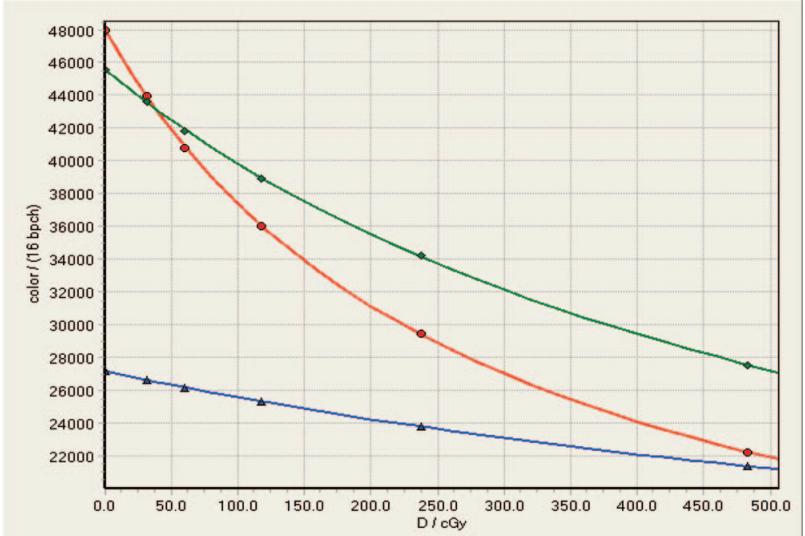
\includegraphics[width=0.5\linewidth]{images/respses.png}
	\caption{Curva de respuesta de película EBT2\cite{manualEBT2}}
	\label{fig:curvaRespuesta}
\end{figure}

Para determinar el cambio de coloración neto de la película se definen las cantidades de transmitancia neta ($netT$) en cada ROI como
\begin{equation}
	netT=T_{irr}-T_{bckg},
\end{equation}
donde $T_{irr}$ es el promedio de transmitancias en la ROI después de la irradiación y $T_{bckg}$ es el promedio de transmitancias en la ROI en la misma película antes de irradiar. Similarmente, se define la densidad óptica neta como 
\begin{equation}
	netOD=OD_{irr}-OD_{bckg},
\end{equation}
donde $OD_{irr}=-\log_{10}T_{irr}$ y $OD_{bckg}=-\log_{10}T_{bckg}$.\\

De esta manera, se construye una relación entre las transmitancias netas o las densidades ópticas netas con las dosis que produjeron la coloración y se ajusta una curva de calibración que permitirá interpolar valores para determinar mapas de dosis a partir de medir densidades ópticas. Un ejemplo de curva de respuesta y curva de calibración para un solo canal se muestra en la figura \ref{fig:Curvas}.

\begin{figure}[H]
	\centering
	\subfloat[Curva de respuesta\cite{Devic2016}]{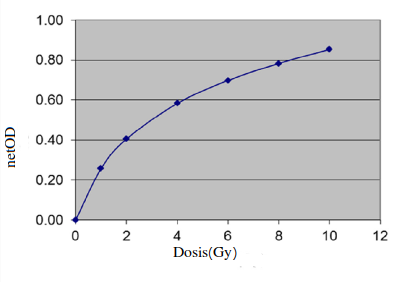
\includegraphics[width=0.5\textwidth]{images/curva1.png}\label{fig:resp}}
	\hfill
	\subfloat[Curva de calibración\cite{Devic2016}]{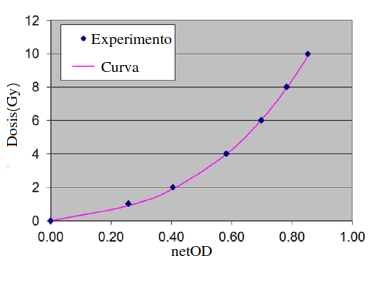
\includegraphics[width=0.5\textwidth]{images/curva2.png}\label{fig:caliv}}
	\caption{Curvas de calibración y respuesta}
	\label{fig:Curvas}
\end{figure}

En la literatura se han propuesto diversos tipo de curva de ajuste para modelar la relación de dependencia observada. Cada una es útil para cierto tipo de película y cierto rango de dosis, por lo que la elección de una en particular depende de la aplicación que se requiera. A continuación se muestran los tipos de funciones más usados\cite{Devic2016} \\

\begin{itemize}
\item\textbf{Función racional}\\
\begin{equation}
	D=\frac{A+B\cdot netT}{netT+D}
\end{equation}
\item\textbf{Función racional cuadrática}\\
\begin{equation}
D=\frac{A+B\cdot netT+C\cdot netT^2}{netT+D}
\end{equation}
\item\textbf{Función cuadrática}\\
\begin{equation}
D=A\cdot netOD^2+B\cdot netOD+C
\end{equation}
\item\textbf{Función cúbica}\\
\begin{equation}
D=A\cdot netOD^3+B\cdot netOD^2+C\cdot netOD +D 
\end{equation}

\item\textbf{Función inversa}\\
\begin{equation}
D=A+\frac{B}{netT-C}
\end{equation}

\item\textbf{Función exponencial}\\
\begin{equation}
D=A\cdot netOD+B\cdot netOD^n
\end{equation}
\end{itemize}

También se han propuesto diversas modificaciones y metodologías para aumentar la precisión de la dosis determinada por la calibración. Cada una de estas tiene en cuenta algún aspecto en particular que altere la medición y lo corrige de cierta manera. A continuación se presentan los principales métodos de corrección.\\


\textbf{Filtrado de las imágenes escaneadas\cite{Devic2005}\cite{Li2017}}\\

Para corregir inhomogeneidades de la película, así cómo irregularidades en la superficie del escáner y pixeles defectuosos se pueden implementar varias correcciones. La más sencilla de ellas es la aplicación de un filtro que elimine outliers de las imágenes, reemplazando su valor por un promedio de los pixeles más cercanos. También se puede escanear varias veces la misma imagen, para luego realizar un promedio ponderado entre ella, eliminando así ciertas irregularidades y reduciendo la incertidumbre teórica que se alcanza.\\

Por otro lado, es común usar un filtro adaptativo de Wiener para reducir el ruido de varias fuentes que puedan tener las imágenes. Este permite eliminar ruido interno producido en la imagen por escaner, como el ruido que se produce en los sensores CCD cuando se están midiendo transmitancias bajas.\\

\textbf{Corrección de efecto lateral} \\

En el caso de usar solo un canal de color para la calibración, en \cite{Crijns2013} se sugiere usar una modificación en la función usada para que tenga en cuenta el efecto de cambio de dosis cerca a los bordes laterales. En la figura \ref{fig:efectoLateral} se evidencia  un ejemplo de este efecto. Esta muestra el perfil de dosis obtenido de una película irradiada uniformemente con una dosis particular, sin embargo en los extremos de la película, los que están cercanos a la parte lateral de escáner, se evidencia una sobre-estimación en la dosis predicha. El efecto sobre la dosis calculada es mayor conforme la dosis aumenta.\\

\begin{figure}[H]
	\centering
	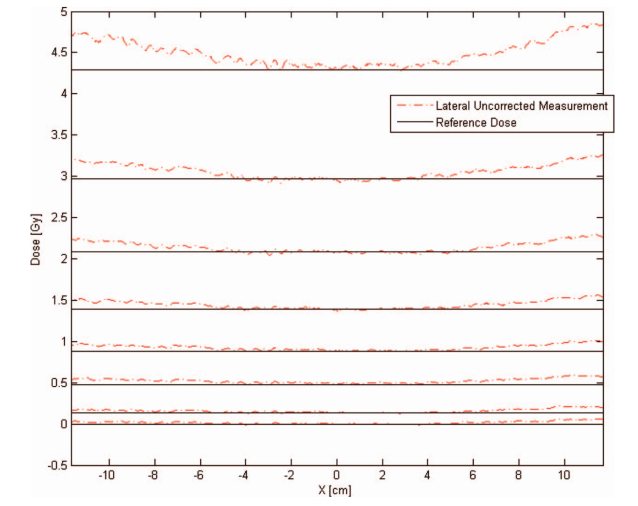
\includegraphics[width=0.9\linewidth]{images/efectoLateral.png}
	\caption{Ilustración del efecto de escaneo lateral para el canal rojo \cite{Crijns2013}}
	\label{fig:efectoLateral}
\end{figure}

Una manera de corregir este efecto es modificar la función de calibración modelando este comportamiento de sobre-estimación. Por ejemplo, si se usa una función racional como las mencionadas anteriormente, una posible modificación modelando el comportamiento del efecto mediante una función cuadrática que tenga como parámetro la variable de posición del escáner, quedando como nueva función
\begin{equation}
	T=T_{\infty}+\frac{T_0-T_{\infty}}{1+\frac{D}{\beta_{3}}}+\beta_{4}D+\beta_{5}X^2,
\end{equation}
donde $T_0, T_{\infty},\beta_{3},\beta_{4},\beta_{5}$ son ahora los nuevos parámetros de ajuste.\\


\textbf{Calibración multicanal}\\

Una manera ingeniosa de mejorar la precisión de las medidas, así como corregir cambios de color no debidos a la dosis absorbida, es usando la información de los tres canales de color como es propuesto en \cite{Micke2011} y expuesto más claramente en \cite{Li2017}. \\

Este método asume que la densidad óptica $(OD)$ en cualquier punto de la película es proporcional al grosor de la capa de material activo
\begin{equation}
	OD_{k}=u_{k}\cdot t \quad k=R,G,B
\end{equation} 
donde $u_k$ es el coeficiente de absorción de la capa activa en cada canal, que varía con la dosis absorbida, y $t$ es una medida adimensional asociada al espesor de la capa activa. Si $f_k$ es la curva de calibración que se está usando para modelar el comportamiento en cada canal, entonces 
\begin{equation}
\label{eqn:cass}
	D_k=f^{-1}(OD_k\cdot t).
\end{equation}

Como la dosis no puede depender del canal de color usado, es posible plantear un problema de optimización en el que variando $t$ se minimizen las diferencias de dosis obtenidas con cada canal, es decir resolver el problema
\begin{equation}
	\min_{t}\sum_{i,j=R,G,B}(D_i-D_j)^2.
\end{equation}

Usando la solución óptima a este problema $t_{opt}$, podemos usar \eqref{eqn:cass} para calcular la dosis en cada canal, y al final tomar el promedio de los resultados en los los tres canales.
\begin{equation}
	D=\frac{D_R+D_G+D_B}{3}
\end{equation}

\section{Análisis $\Gamma$}
Dada la complejidad que suponen ciertos tratamientos y la necesidad de asegurar que las dosis prescritas correspondan con gran precisión con las dosis entregadas en estos, se deben proponer formas cuantitativas para evaluar qué tanto corresponden entre sí dos mapas de dosis asociados a los planes. Esto se requiere, por ejemplo, cuando por diversas razones es necesario cambiar el algoritmo de cálculo de dosis que usa el sistema de planeación para calcular los planes. En tal caso, es necesario validar el reajuste con los planes previamente calculados, para asegurar que correspondan con las dosis prescritas.\cite{Winiecki2009}\cite{Li2011}\\

En este caso, se quiere validar que los planes calculados con el sistema de planeación correspondan con los que se ejecutan en tiempo real en la máquina. Esto dado que, en algunos casos, para planes complejos, las limitaciones de la máquina que no tiene en cuenta el sistema podrían generar distribuciones inciertas que afectan la efectividad del tratamiento.\\

En consecuencia, para propósitos de comparación de planes, se ha desarrollado una nueva cantidad denominada $\Gamma$. Si se desea comparar una distribución de dosis de referencia $D(\vec{r}_{c})$ con una distribución de dosis medida $D(\vec{r}_{m})$ entonces se define $\Gamma(\vec{r}_c,\vec{r}_m)$ para cada punto de referencia con respecto a cada punto de medida como 
\begin{equation}
\label{eqn:gamma}
\Gamma(\vec{r}_c,\vec{r}_m)=\sqrt{\frac{\abs{\vec{r}_c-\vec{r}_m}^2}{DTA^2}+\frac{\abs{D(\vec{r}_c)-D(\vec{r}_m)}^2}{DD^2\cdot D(\vec{r}_c)^2}},
\end{equation}
donde $\abs{\vec{r}_c-\vec{r}_m}$ es la distancia entre los puntos analizados en milímetros, ${\abs{D(\vec{r}_c)-D(\vec{r}_m)}}$ es la diferencia de dosis entre los puntos y $DTA$(Distance to Agreement) y $DD$(Dose diference) son parámetros para ajustar la calidad de la comparación. Teniendo estos valores, se define el valor de $\Gamma$ en cada punto de la distribución de referencia como el mínimo de estas cantidades evaluadas sobre los puntos en la distribución de mediada, es decir $\Gamma(\vec{r}_c)=\min_{m} \Gamma(\vec{r}_c,\vec{r}_m)$.\\

De esta manera, para $DTA$ y $DD$ fijos, se está buscando en la distribución medida el punto que está más cercano en una distancia de hasta $DTA$ y difiere en dosis hasta $DD$ con respecto a algún punto en la distribución de referencia. Parámetros usuales para realizar este análisis son $DTA=3 mm$ y $DD=3.3\%$, aunque para planes más complejos, con gradientes de dosis altos, se pueden usar parámetros menores, como $DTA=1 mm$ y $DD=1\%$.\\

Cada punto en la distribución de referencia pasa el test de comparación con la distribución medida si su $\Gamma(\vec{r}_c)<1$, lo que quiere decir que, bajo la definición de comparación de distribuciones, estas coinciden en un valor aceptable. Gráficamente, el significado de este test de ajuste entre distribuciones es representado en la figura \ref{fig:elipseGamma}, donde un punto en la distribución de referencia pasa el test si reside en la elipse  definida por la ecuación \eqref{eqn:gamma}.\\
\begin{figure}
	\centering
	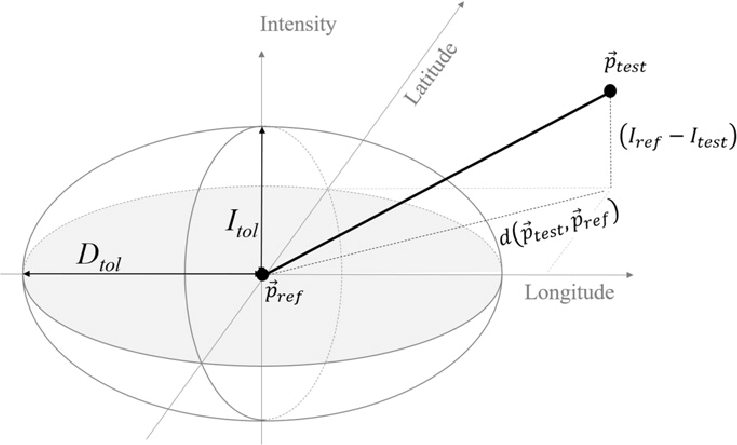
\includegraphics[width=0.5\linewidth]{images/gammaEllipse.png}
	\caption{Significado geométrico del test gamma }
	\label{fig:elipseGamma}
\end{figure}







\chapter{Metodología}\label{chp:metodologia}
En esta sección, se describe el procedimiento para obtener la curva de calibración que se usó, así como detalles técnicos del montaje experimental y los implementos que se requirieron. 
\section{Procedimiento de irradiación}
Los procedimientos de irradiación se realizaron con un acelerador True Bream de  Varian, operado a 6 $ MeV$ con filtro aplanador. Este acelerador fue calibrado con cámara de ionización siguiendo el protocolo TRS 398 para comprobar la fiabilidad de que la dosis entregada correspondiera con las unidades monitor requeridas. Una fotografía del montaje usado en el procedimiento se muestra en la figura \ref{fig:fotoMontaje}.\\

\begin{figure}
	\centering
	% \missingfigure is from todonotes
	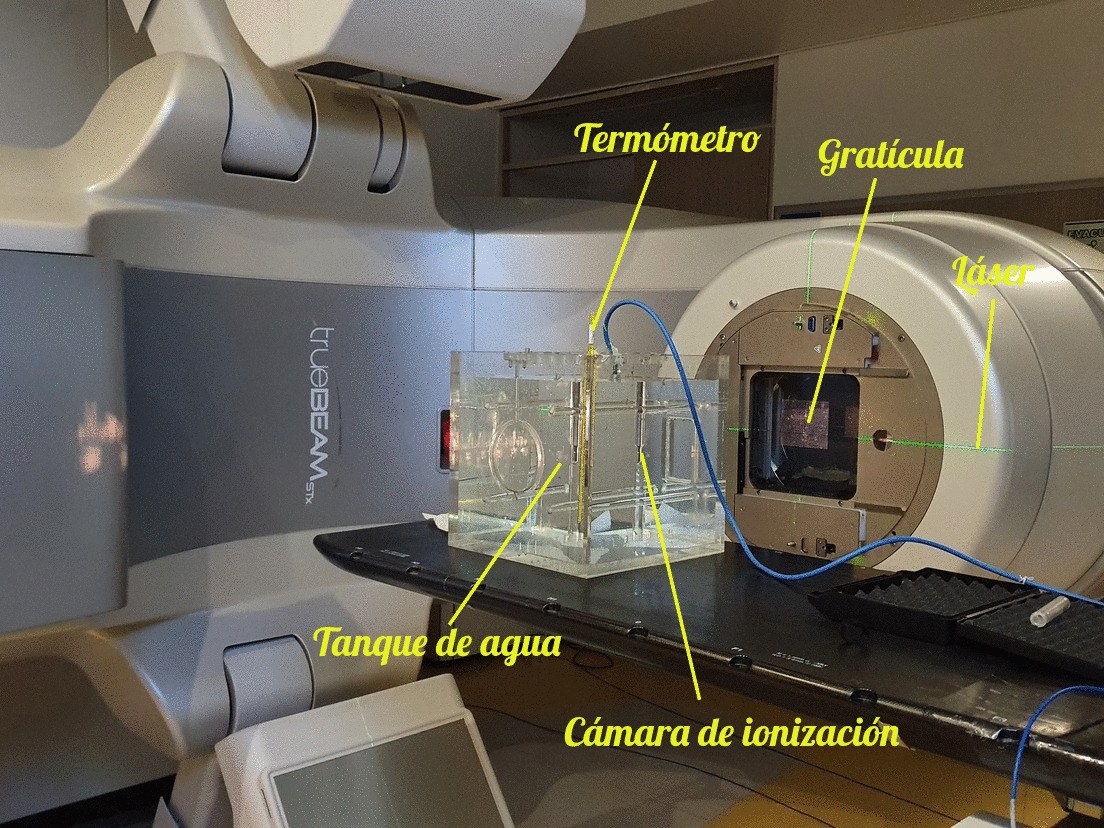
\includegraphics[width=0.7\linewidth]{images/TRS398Editado2.jpg}
	\caption{Montaje de calibración del acelerador.}
	\label{fig:fotoMontaje}
\end{figure}
Para obtener la curva, se irradiaron fragmentos de películas EBT3 del mismo lote de aproximadamente 5 cm x 5 cm, cortados manualmente con un bisturí. El proceso de corte despega la lamina protectora de la película, por lo que se debe tener en cuenta no usar las regiones cercanas al corte en la obtención de medidas para la calibración, puesto que cambian las propiedades ópticas con respecto a la región lejana al corte. Por otro lado, toda manipulación de las películas se realizó con guantes de nitrilo para no dejar residuos que podrían tener cierto efecto en la medida de la transmitancia. \\

Para la irradiación se alineó, con la ayuda de luz de campo, la gratícula del acelerador, los láseres del cuarto de tratamiento, y el telémetro incorporado en el acelerador, cada trozo de película con el isocentro del acelerador. Cada película fue irradiada en el centro de un campo de 20 x 20 cm a 100 cm del foco para lograr uniformidad de campo en la región donde se encuentra la película. Además, se usaron 5 cm de agua sólida PTW/IBA encima de la película y 5 cm debajo de ella para tener en cuenta efectos de la retro dispersión de la radiación. En la figura  \ref{fig:MontajePelicula} se muestra el montaje usado para la irradiación en el caso de la película sin recortar.\\
\begin{figure}
	\centering
	% \missingfigure is from todonotes
	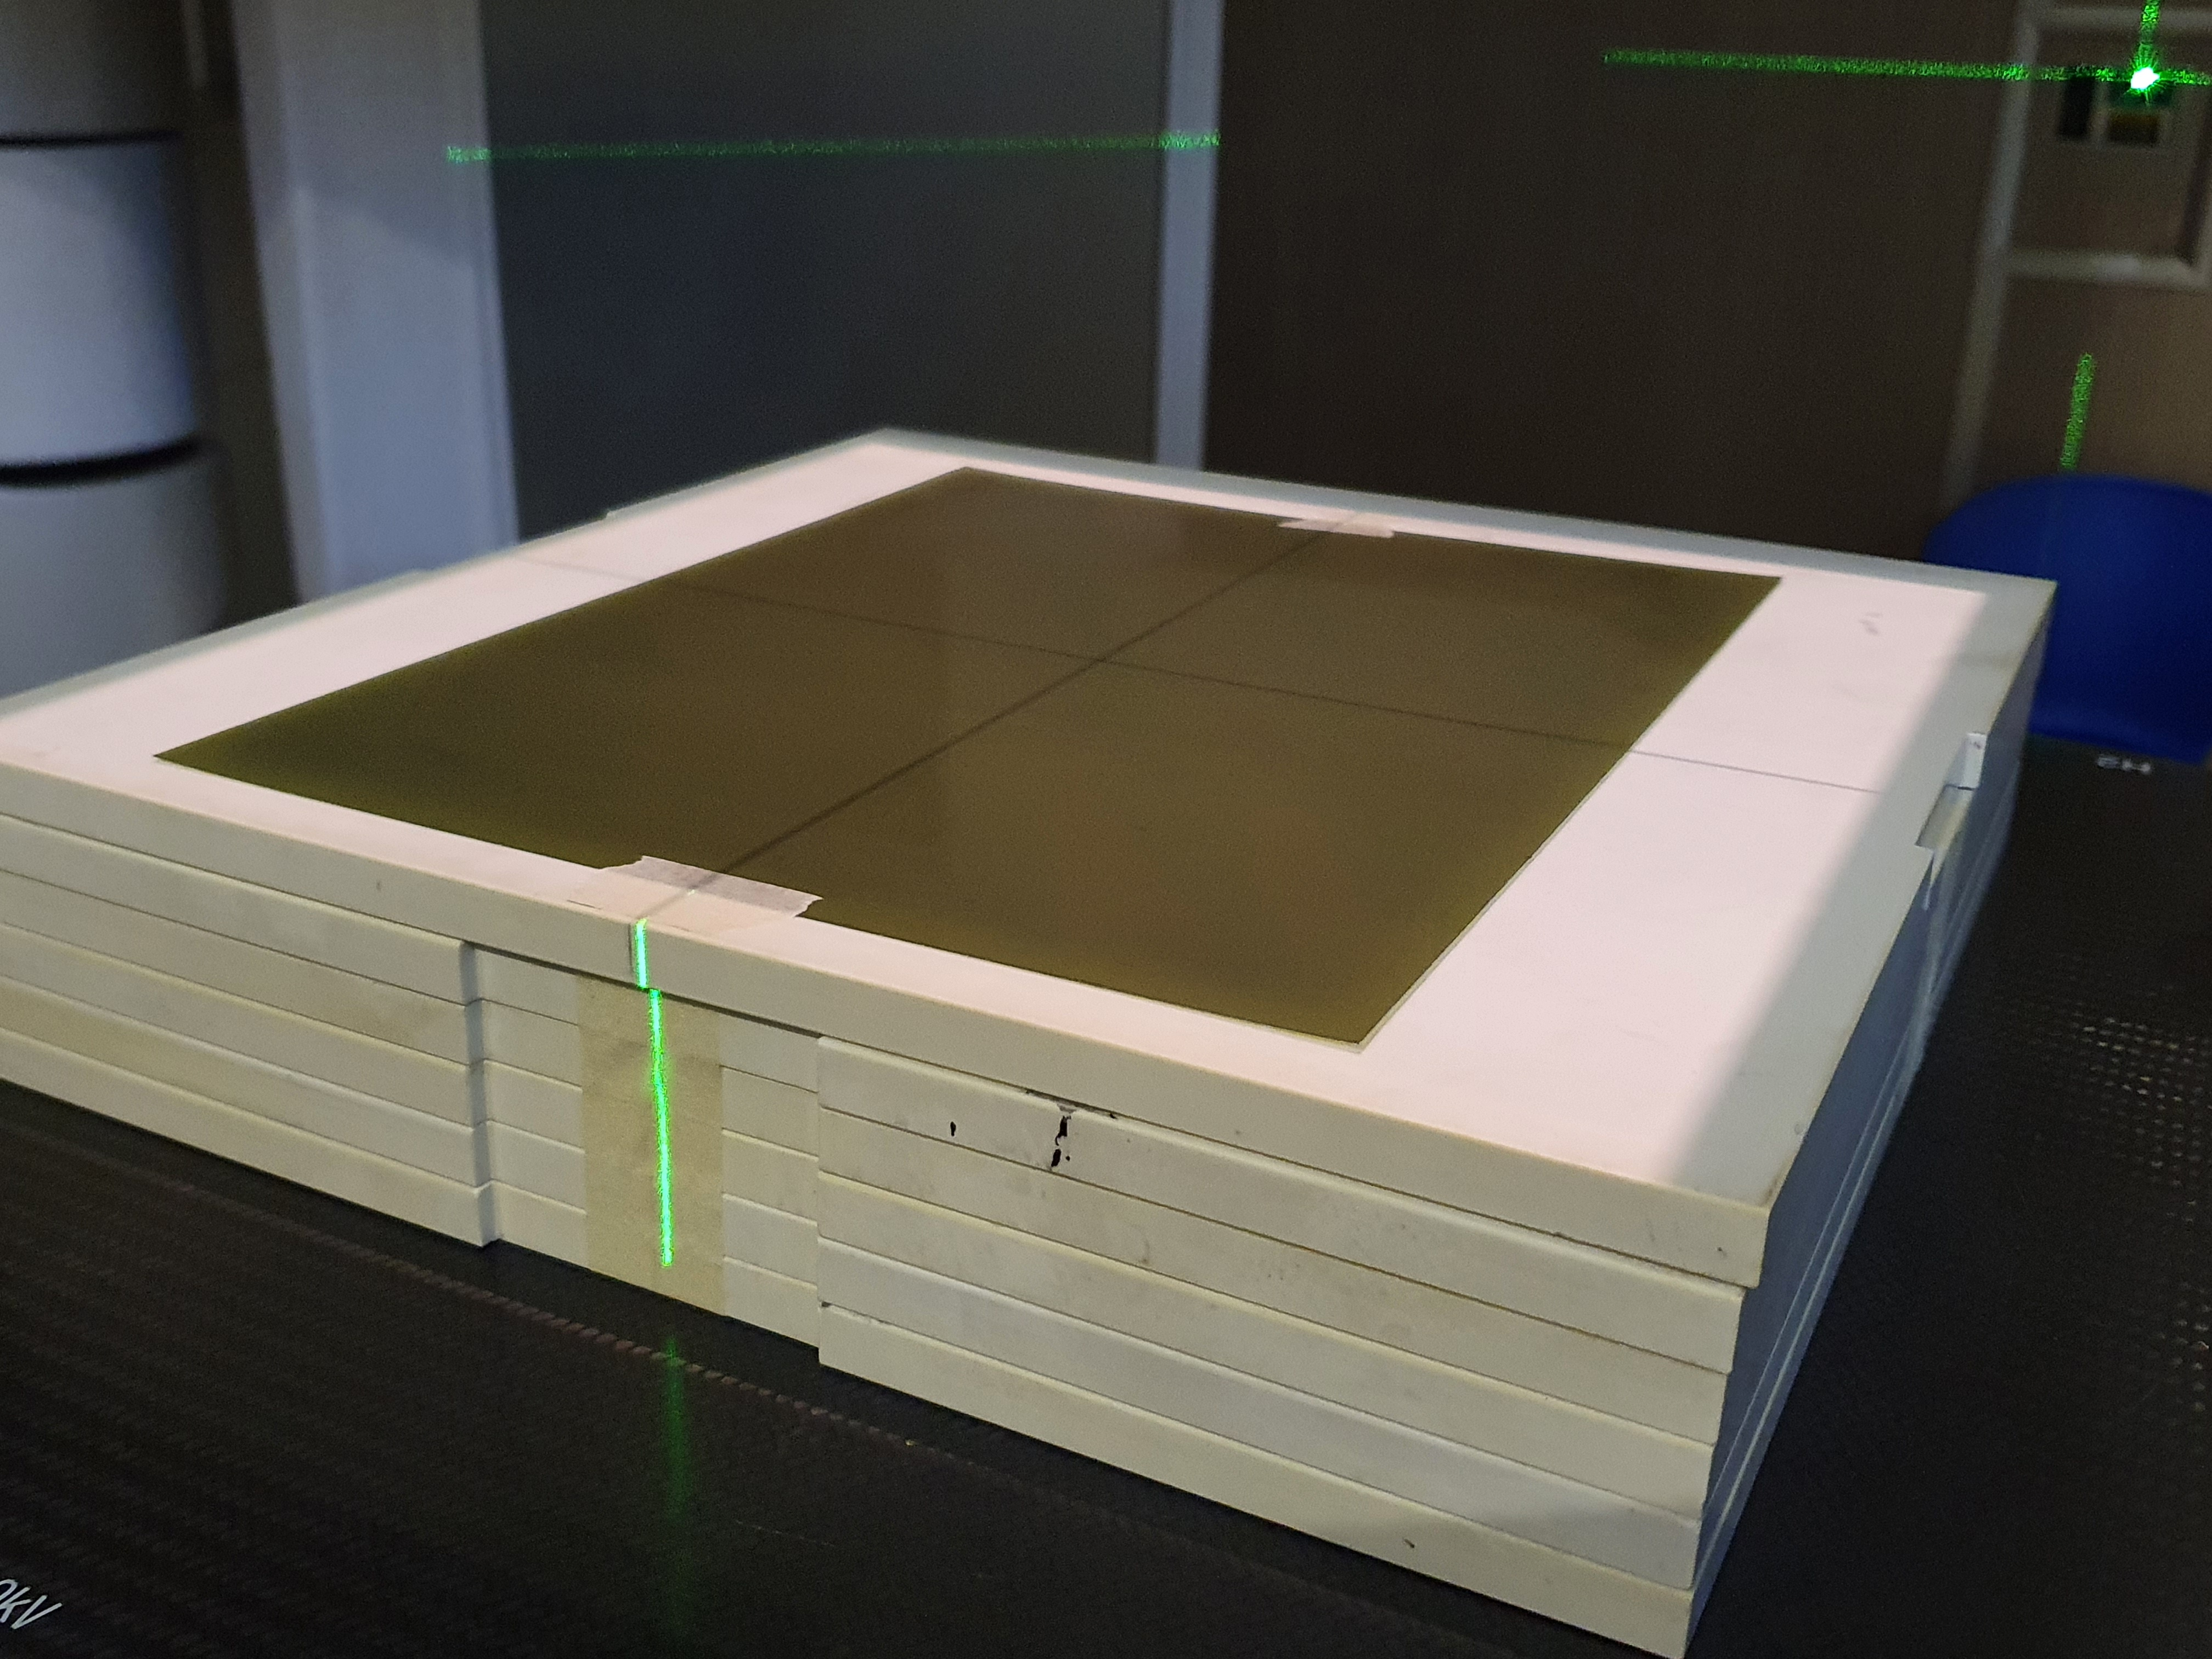
\includegraphics[width=0.7\linewidth]{images/alineacionCampo.jpg}
	\caption{Alineación de la película ajustada con el isocentro del acelerador.}
	\label{fig:MontajePelicula}
\end{figure}

Con el objetivo de medir los cambios de coloración que se dan debido a la radiación, se planeó irradiar películas con dosis entre 0 y 20 Gy. Con el objetivo de comprobar que el cambio de color fuera unívocamente correspondiente a la dosis depositada, por cada dosis elegida se irradiaron tres películas, para luego comparar su cambio de coloración y determinar si se reproduce el mismo cambio en las tres.\\ 


Para determinar experimentalmente las dosis que se irradiaron, se usó un montaje con una cámara de ionización Farmer 30010 PTW Freiburg GmbH junto con un electrómetro, siguiendo el protocolo TRS398 descrito anteriormente. Así, por cada cantidad fija de unidades monitor que se programaron con la máquina, se realizó la medición de la dosis efectiva depositada a la misma profundidad de agua solida y distancia a la fuente que se usó en la irradiación de las películas. Esta medición se realizo diez veces para las primeras cuatro dosis, siete veces para la quinta dosis, cinco veces para las siguientes tres y finalmente tres veces para las últimas tres dosis. El montaje de lectura con el electrómetro se muestra en la figura \ref{fig:Montajeelectrometro}\\
\begin{figure}[H]
	\centering
	% \missingfigure is from todonotes
	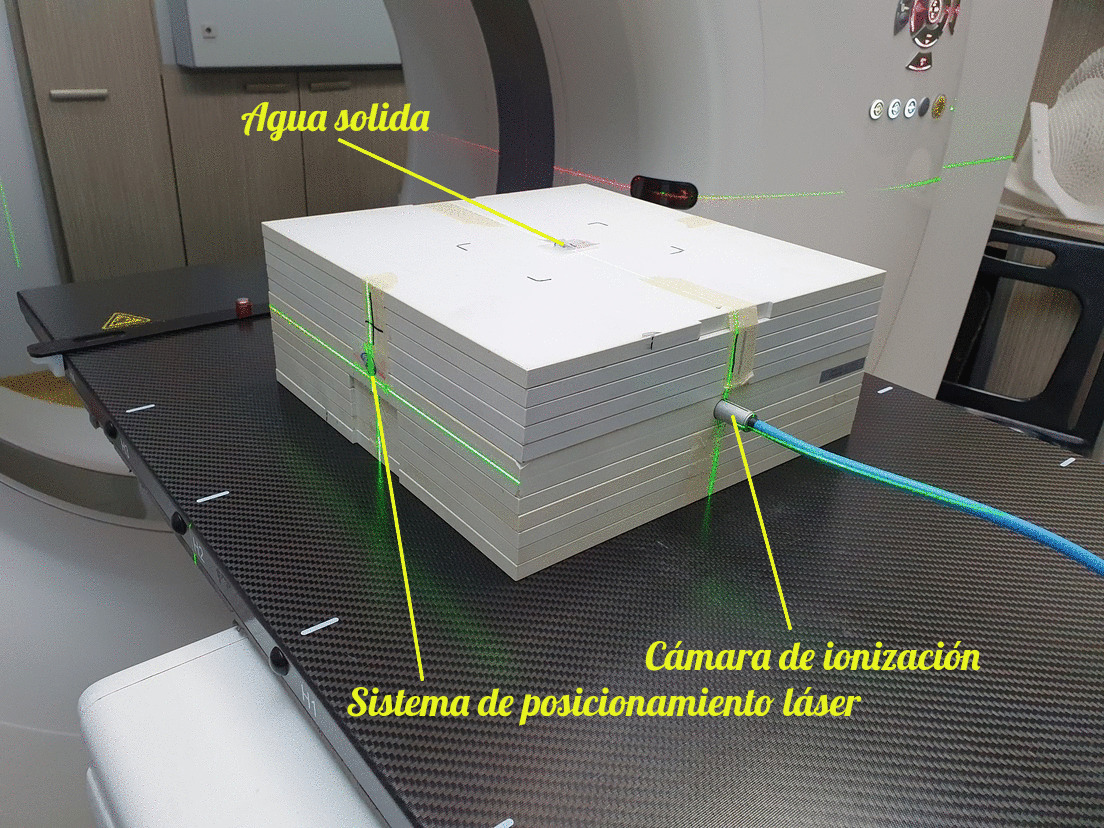
\includegraphics[width=0.7\linewidth]{images/elctrometro.jpg}
	
	\caption{Montaje para determinación de dosis.}
	\label{fig:Montajeelectrometro}
\end{figure}

La cantidad de unidades monitor que se requieren entregar para lograr determinada dosis absorbida en el plano de la película se calcularon mediante el sistema de planeación Eclipse\footnote{https://www.varian.com/es/products/radiotherapy/treatment-planning/eclipse}. Para esto se tomó un TAC del agua solida y la cámara de ionización y se reconstruyó la geometría bajo la cual fueron realizados los cálculos.\\

Por otro lado, para realizar comparaciones entre mapas de dosis de tratamientos calculados con el sistema de planeación y los mapas de dosis obtenidos mediante la calibración, se irradiaron dos planes. En primer lugar, se irradió un plan pirámide, que en el plano de la película produce un mapa de dosis calculado por el sistema como se ilustra en la figura \ref{fig:TPSPiramide}\\

\begin{figure}
	\centering
	% \missingfigure is from todonotes
	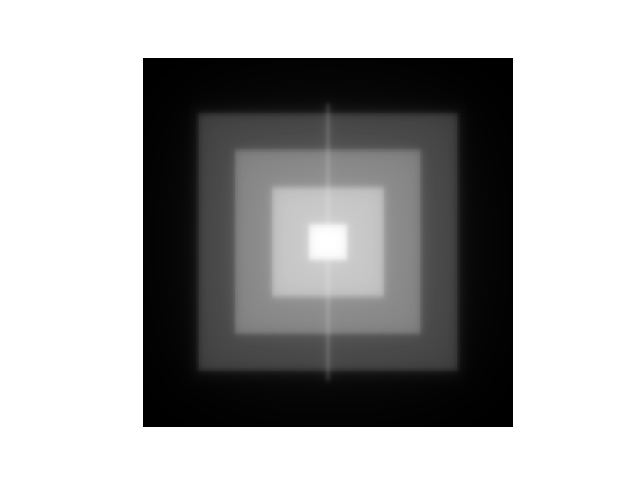
\includegraphics[width=0.7\linewidth]{images/piramideTPS.png}
	\caption{Mapa de dosis calculado por el sistema de planeación en el plano de la película para el plan pirámide.}
	\label{fig:TPSPiramide}
\end{figure}

Posteriormente, se irradió un plan de tratamiento IMRT de cáncer de mama colapsado a 0°, es decir, todos los campos del plan fueron irradiados de forma perpendicular a la película. Este plan produjo un mapa de dosis en el plano de la película calculado por el sistema de planeación que se ilustra en la figura \ref{fig:TPSMama}\\

\begin{figure}
	\centering
	% \missingfigure is from todonotes
	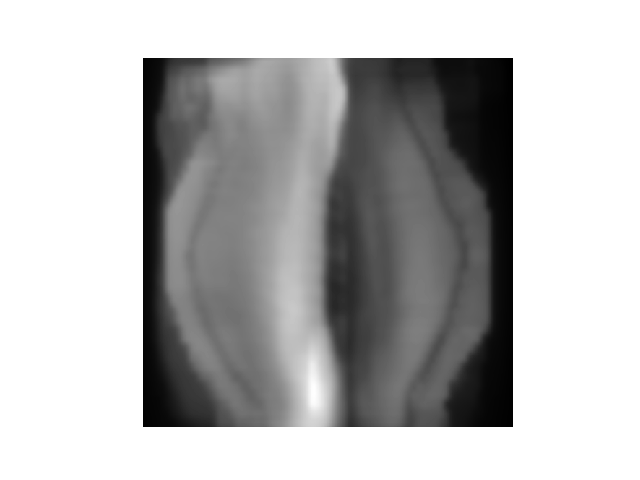
\includegraphics[width=0.7\linewidth]{images/mamaTPS.png}
	\caption{Mapa de dosis calculado por el sistema de planeación en el plano de la película para el plan de tratamiento de mama.}
	\label{fig:TPSMama}
\end{figure}

Por otro lado, también se irradió un cuadrado con 5 Gy, usando las láminas del MLC para formar un campo de 10 x 10 cm, para realizar la comprobación más sencilla de la eficiencia del proceso de calibración.\\

Finalmente, se calcularon los mapas de dosis obtenidos mediante las películas y se compararon con los mapas calculados usando diversas herramientas, incluyendo el análisis $\Gamma$.

\section{Escaneo y tratamiento}
Para la fase de digitalización se usó un escáner ScanMaker 1000XL en modo de transmisión que tiene un área operativa de 30.48 cm x 40.64 cm, eligiendo el modo RGB con 16 bits por canal, desactivando los filtros y correcciones automáticas y usando una resolución de 100 ppi siguiendo las recomendaciones propuestas en \cite{Devic2016}. Con esta configuración, se obtienen imágenes a color en formato TIFF de alrededor de 10 MB de tamaño, dependiendo del tamaño del área escaneada. Esta imagen, sin ningún tipo de compresión, se puede traducir a una matriz de pixeles con valores entre $0$ y $2^{16}-1$, por cada canal de color, que puede ser leída mediante diferentes paquetes de programación. En este caso, se usa la librería de python tiffread para la lectura. \\



En la figura \ref{fig:fondoNegro} se muestra una imagen del escáner cuando la lámpara fue opacada con abundante cartulina negra. Para corregir estos pixeles, se usó una combinación entre las técnicas de supresión de ruido con background y filtrado con filtros de Wiener y mediana. \\

Para reducir efectos de dependencia de posición, se usó siempre la parte central superior del escáner para digitalizar las imágenes. De esta manera, el sesgo sería siempre el mismo y podría ser corregido con el método multicanal propuesto.\\

En \cite{Micke2011} se reporta que este método para predecir dosis aporta en la separación de cambios de color debidos a defectos del escáner y cambios de color debidos a la irradiación propiamente. En la figura \ref{fig:Multicanal} se evidencia como el uso de este método puede usarse para separar la parte dependiente de la dosis del color de la parte que es dependiente de las heterogeneidades del escáner, en este caso se usa el ejemplo propuesto en \cite{Micke2011}. \\

\begin{figure}
	\centering
	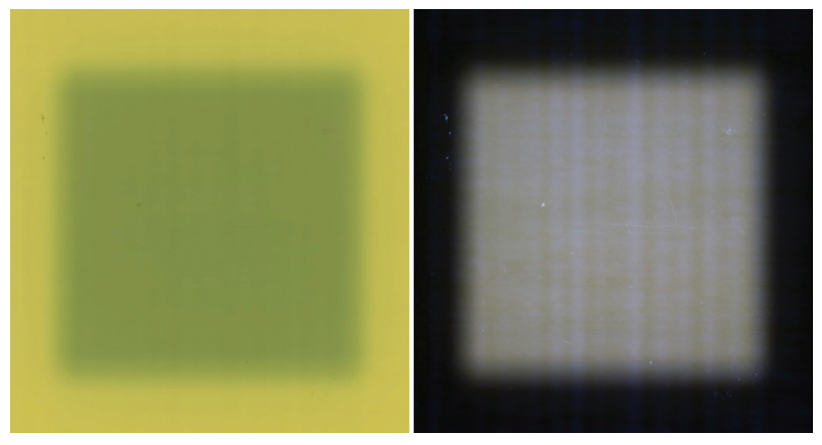
\includegraphics[width=0.7\linewidth]{images/imagenMicke.png}
	
	\caption{Separación de parte dependiente de dosis\cite{Micke2011}.}
	\label{fig:Multicanal}
\end{figure}

Además, para corregir este efecto de mejor manera, el programa también incluye la opción de restar el sesgo a cada medida a partir de una medida de una película sin irradiar. De esta manera, el cambio de coloración es ajustado con respecto a como varía la respuesta en función de la ubicación escaneada. \\

De la misma manera, se implementó el uso de filtros para corregir particularidades del escáner como pixeles dañados y rayones en la película o escáner. El filtro recomendado en la literatura para estas circunstancias es el filtro de Wiener \cite{Devic2016}, el cual se implementó en el programa. \\

También, es posible usar el filtro en el cual el valor de transmitancia en cada pixel se remplaza con el promedio de los valores que lo rodean, eliminando parcialmente ciertas inhomogeneidades que podrían presentarse. Otro filtro posible es el filtro de mediana, que reemplaza en cada pixel su valor por el que más se repite a su alrededor en cierto intervalo. \\

La eficiencia de estos filtros es dependiente de la calidad de la imagen obtenida, por lo que para cada digitalización se probaron diferentes combinaciones de estos, siendo los más eficientes, en la mayoría de los casos, el filtro de la mediana y el filtro de Wiener.\\

Aunque la aplicación de filtros ayuda de cierta manera a reducir los efectos de las heterogeneidades de fabricación, estos no lo solucionan por completo, puesto que estas son de carácter no local. La mejor manera de incrementar la seguridad con respecto a este tipo de incertidumbre es realizando varias irradiaciones en  diferentes películas y comparando sus resultados.\\


Por otro lado, el fabricante del lote de películas EBT3 usado reporta que en el último control de calidad realizado, las películas presentaban una homogeneidad superior al 95 \% sobre su superficie, es decir, la estructura física de la película podía variar 5\% en sus dimensiones en algunas secciones. Esto no implica directamente una desviación de más de 5\% en el color medido por esta inhomogeneidad, puesto que la capa activa permanece generalmente uniforme, pero si afecta de cierta manera relativamente sutil la medida. Este efecto también puede ser corregido mediante el método multicanal. \\ 



Finalmente, para evitar cambios en la medida por efectos de la orientación de la película en el escáner, se escaneó siempre usando la orientación horizontal en la parte superior del escáner.\\

\section{Programa para el análisis de películas}

Para ejecutar el análisis de películas radiocrómicas irradiadas usando diversas técnicas mencionadas anteriormente, como métodos de calibración y corrección, y de manera efectiva se implementó un programa en el lenguaje de programación Python. \\

Este programa permite usar diversas herramientas para el análisis de estas películas, las cuales se pueden dividir en cuatro categorías generales.\\

El primer conjunto de herramientas permite generar curvas de calibración a partir de imágenes digitalizadas de películas irradiadas con una dosis conocida. Esta sección permite elegir el tipo de curva usada, así como la elección de los canales a usar. Para elegir la transmitancias promedio el programa permite seleccionar ROIs, áreas en las cuales se promedia el valor de los tres canales de color. También permite promediar los colores de múltiples películas irradiadas con la misma dosis para mejorar la calidad de la medida. El resultado de la función de la calibración persiste como un archivo en formato .calibr, el cual contiene toda la información que se usó para generar la curva.\\

El segundo conjunto de herramientas permite generar mapas de dosis a partir de una película escaneada y un archivo de calibración, además de proporcionar algunas herramientas para analizar estos mapas. Se incluyen funciones como reducir el tamaño del área de interés, elegir y remover puntos fiduciales en la sección de la película, mostrar mapas de isodosis y perfiles e histogramas de dosis, así como elegir la normalización sobre la que se calcularon. El mapa final se guarda en  un archivo en formato DICOM.\\

El tercer conjunto de herramientas permite realizar comparaciones plan-película con análisis $\Gamma$ a partir de dos archivos en formato DICOM, uno correspondiente al plan calculado por el TPS y otro generado en el paso anterior con la información de la película. En este conjunto se incluyen herramientas como la superposición de mapas de isodosis y perfiles de dosis, así como visualizaciones propias del análisis $\Gamma$, como la matriz y el histograma $\Gamma$, además del porcentaje de aprobación del test.\\

Por último, en la cuarta categoría se encuentran herramientas auxiliares para facilitar el uso del programa. Entre estas se incluyen la elección de los filtros usados, la elección de las propiedades del escáner , herramientas para apilar y reflejar imágenes, entre otras.\\

Una descripción más detallada del programa puede encontrarse en los apéndices A y B.





  












\chapter{Resultados y análisis}\label{chp:resultados}
En esta sección se presentan resultados obtenidos para la calibración usada, así como la obtención y análisis de mapas de dosis obtenidos.
\section{Calibración}
Como fue mencionado anteriormente, se irradiaron películas con dosis que se registran en la tabla \ref{tab:DosisIrra}, con su correspondiente incertidumbre, medidas con la cámara de ionización.

\begin{table}[]
	\centering
	\begin{tabular}{|l|l|l|}
		\hline
		UM& Dosis(Gy)    & Incertidumbre($10^{-5}$) \\ \hline
		21.6&0.201472 & 3.8\\ \hline
		54&0.504137 & 5.23 \\ \hline
		108&1.00825  & 35\\ \hline
		216&2.01783  & 22\\ \hline
		432&4.037486 & 31 \\ \hline
		648&6.0583   & 48\\ \hline
		864&8.08168  & 142\\ \hline
		1080&10.1056  & 140\\ \hline
		1296&12.132   & 10\\ \hline
		1620&15.168   & 10\\ \hline
		2160&20.229   & 10\\ \hline
	\end{tabular}
	\caption{Dosis irradiadas}
	\label{tab:DosisIrra}
\end{table}

Las películas resultantes después de la irradiación se muestran en la figura \ref{fig:peliculasIrradiacion}. Todas las películas fueron escaneadas en la misma sección del escaner para reducir efectos de posición en la transmitancia.\\
\begin{figure}[H]
	\centering
	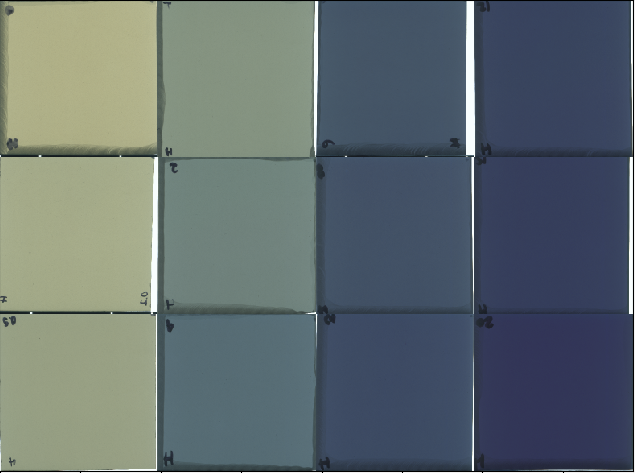
\includegraphics[width=0.7\linewidth]{images/peliculasIrradiadas.png}
	\caption{Películas EBT3 irradiadas con dosis entre 0 y 20 Gy }
	\label{fig:peliculasIrradiacion}
\end{figure}

Para relacionar determinados niveles de transmitancias medidas en una película con la dosis que produjo la coloración es necesario establecer una curva de calibración. En este caso se correlacionaron los promedios de transmitancia en regiones de interés de las tres películas irradiadas con la misma dosis con la dosis medida con la cámara de ionización que produjo dicha coloración. Con estos valores se establece la curva de calibración que se muestra en la figura \ref{fig:curvaFinal20} con sus respectivos parámetros.\\


\begin{figure}[H]
	\centering
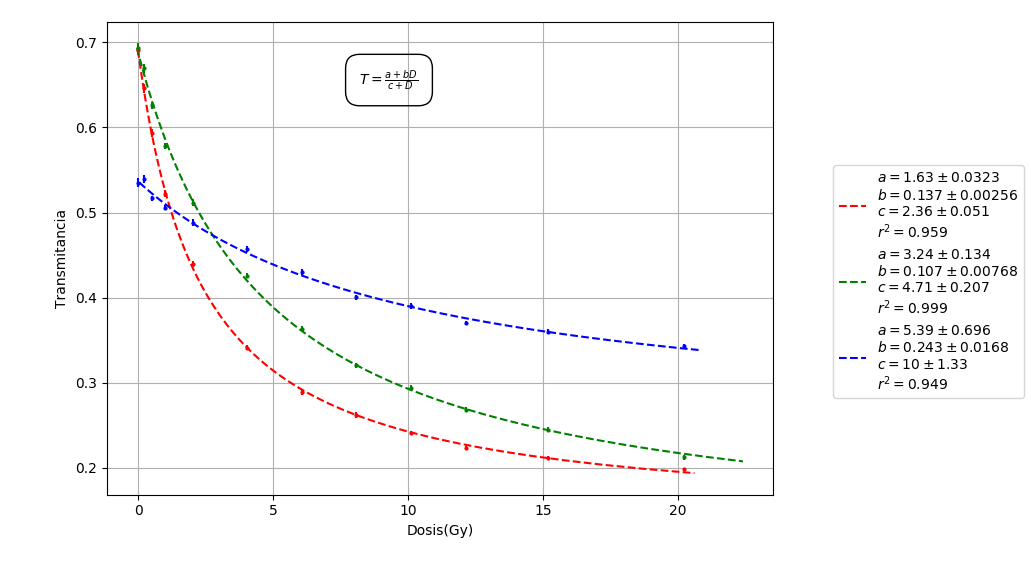
\includegraphics[width=\linewidth]{images/calibracionMulti0a20.png}
	
	\caption{Curva de calibración con dosis de 0 a 20 Gy }
	\label{fig:curvaFinal20}
\end{figure}

En la cual se usó una curva del tipo 
\begin{equation}
D=\frac{AT+D}{T-C}.
\end{equation}\\

Según el manual del fabricante, las películas EBT3 son aptas para un rango inferior a 10 Gy, por lo que se prefieren omitir los últimos tres puntos de dosis, puesto que la película está en la región de saturación en esta región.  Además, estos puntos no aportan información adicional a los propósitos del trabajo, puesto que los planes que serán examinados no conllevan dosis tan altas. De esta manera se obtiene la curva que se muestra en la figura \ref{fig:curvaFinal}\\

\begin{figure}[H]
	\centering
	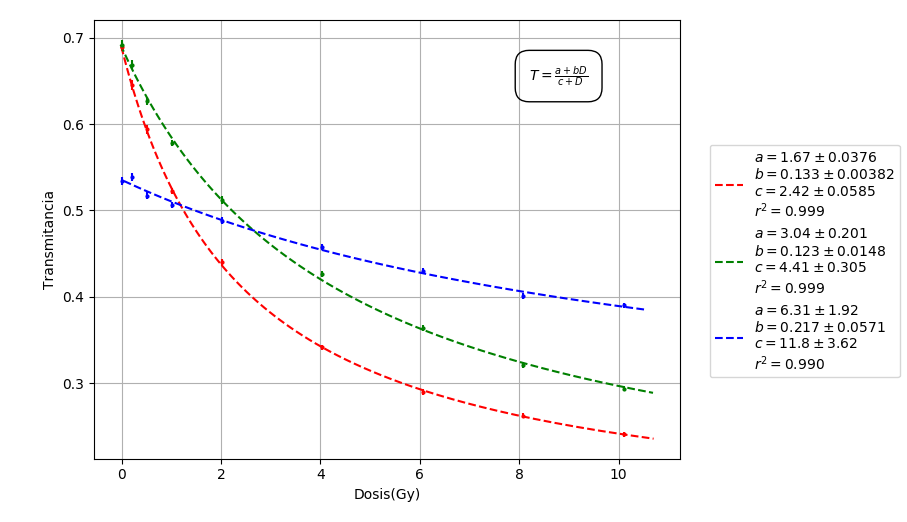
\includegraphics[width=\linewidth]{images/calibracionMulti.png}
	\caption{Curva de calibración con dosis de 0 a 10 Gy }
	\label{fig:curvaFinal}
\end{figure}

En esta se evidencia que las curvas ajustadas describen mejor los datos puesto que no se ha alcanzado la región de saturación, lo cual se demuestra con los mejores test de ajuste $\chi ^2$ calculados. También se evidencia que el canal que menos se ajusta y tiene un comportamiento más por fuera de lo esperado es el azul, consecuente con el hecho que en esta longitud de onda los cambios de coloración de la película son menores. Estas curvas son las que se usan a lo largo del trabajo para calcular mapas de dosis.\\

También se probaron más curvas sugeridas en la literatura, sin embargo, la que mejor se ajustó a los datos con las películas EBT3 en este rango de dosis fue la anteriormente mencionada. En la figura \ref{fig:CurvasAdicionales} se muestran otros dos ajustes con las respectivas formas de la función de ajuste y su bondad de ajuste.


\begin{figure}[H]
	\centering
	\subfloat[Curva cubica]{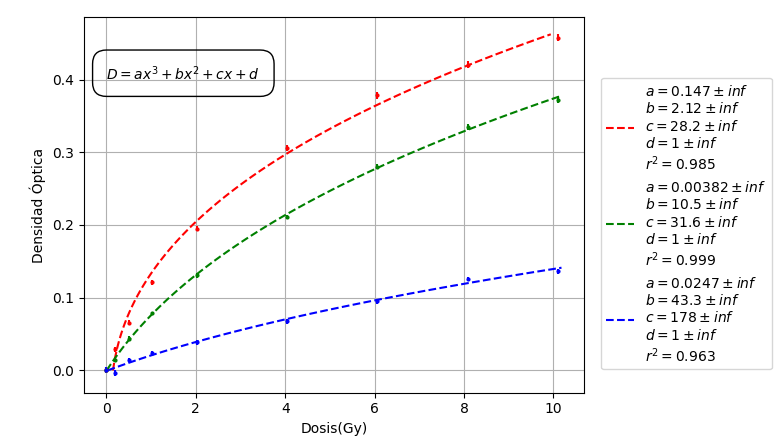
\includegraphics[width=0.7\textwidth]{images/calibracionCubica.png}\label{fig:cubic}}
	\hfill
	\subfloat[Curva exponencial]{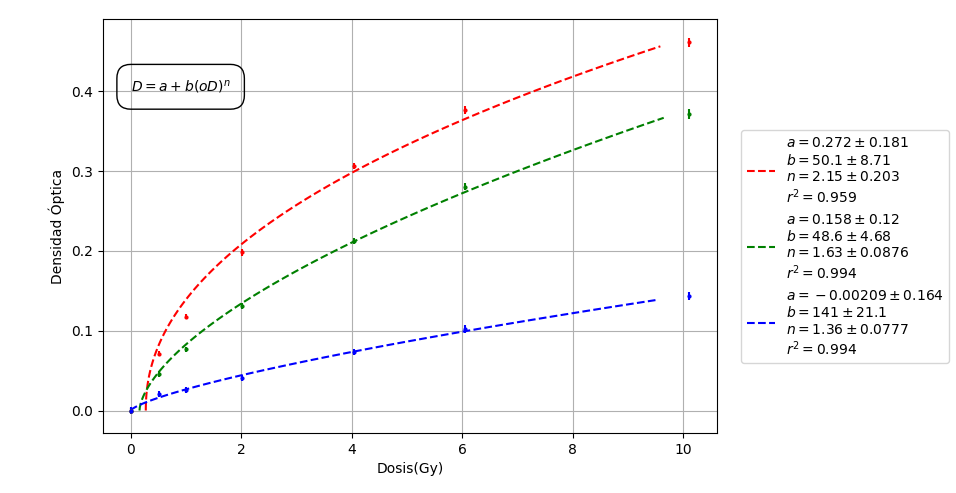
\includegraphics[width=0.7\textwidth]{images/curvaCalibracionMalaExponencial.png}\label{fig:expo}}
	\caption{Curvas de calibración con otro tipo de funciones}
	\label{fig:CurvasAdicionales}
\end{figure}

Acá la curva \ref{fig:cubic} se ajustó a una función cúbica, pero no se pudieron estimar las incertidumbres en los coeficientes por una razón desconocida. Similarmente, en la curva \ref{fig:expo} se realizó un ajuste a una función exponencial que resulto de menor calidad comparado con la función racional usada inicialmente. Se debe notar que en este caso las curvas relacionan las cantidades  de densidad óptica con dosis absorbida y no de transmitancia directamente.\\

Finalmente, la única curva para realizar el  procedimiento de calibración multicanal fue la curva propuesta inicialmente, esto dado que las demás son susceptibles a errores numéricos que causan inestabilidad en el método de minimización usado.


\section{Efectos de diversos parámetros}

Para evaluar los efectos de diversos factores en la digitalización y posterior conversión de películas radicrómicas en mapas de dosis se estudiaron varios ejemplos. \\

En primer lugar, se estudió el efecto de la posición en el área de escaneo en la transmitancia medida con el escáner. Para esto se examina el comportamiento de la transmitancia de una película sin irradiar a lo largo de un perfil horizontal y vertical en esta. Con este objetivo, la digitalización de la placa que se muestra en la figura \ref{fig:fondoCero} se transformó en un mapa de dosis al cual se le extrajeron los perfiles horizontales y verticales que se muestran en la figura \ref{fig:perfiles}.\\

\begin{figure}[H]
	\centering
	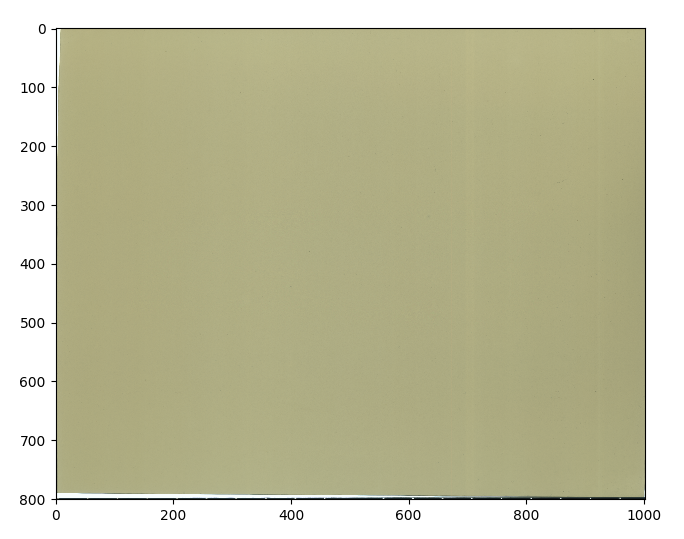
\includegraphics[width=0.7\linewidth]{images/imagenFondoCero.png}
	\caption{Curva de calibración con dosis de 0 a 10 Gy }
	\label{fig:fondoCero}
\end{figure}

\begin{figure}[ht] 
	\centering
	\begin{minipage}[b]{0.6\linewidth}
		\centering
		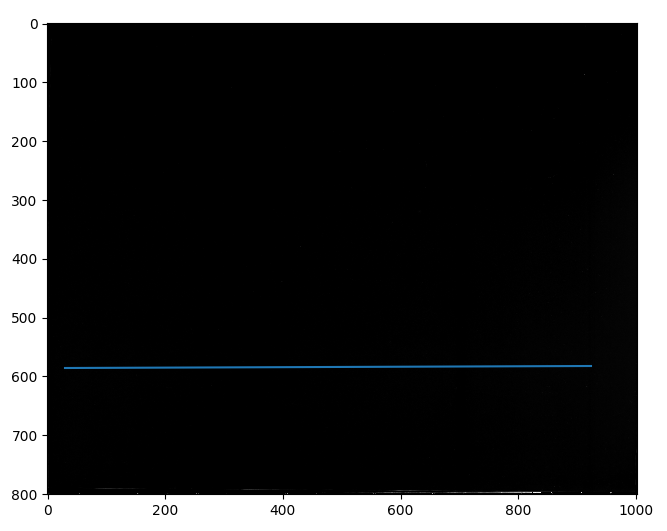
\includegraphics[width=.5\linewidth]{images/imagenPerfilMapaCeroHorizontal.png} 
		\caption{Perfil horizontal} 
		\label{fig:perhor}
		\vspace{4ex}
	\end{minipage}%%
	\begin{minipage}[b]{0.6\linewidth}
		\centering
		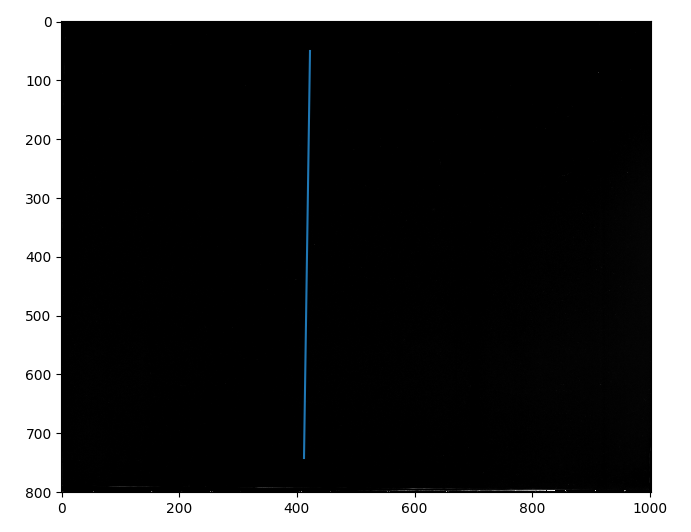
\includegraphics[width=.5\linewidth]{images/imagenPerfilMapaCeroVertical.png} 
		\caption{Perfil vertical} 
		\vspace{4ex}
	\end{minipage} 
	\begin{minipage}[b]{0.6\linewidth}
		\centering
		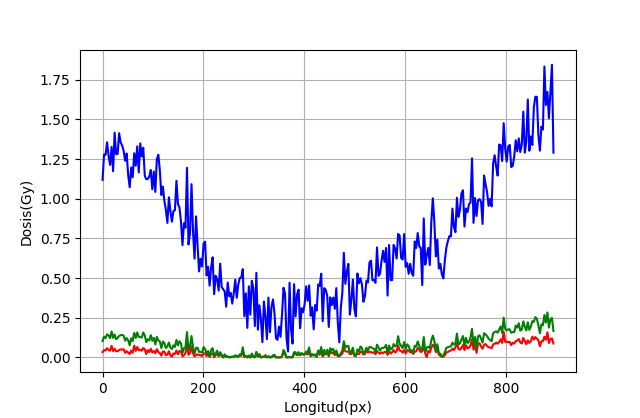
\includegraphics[width=.5\linewidth]{images/perfilDosisCeroHorizontal.png} 
		\caption{Perfil de dosis horizontal} 
		\vspace{4ex}
	\end{minipage}%% 
	\begin{minipage}[b]{0.6\linewidth}
		\centering
		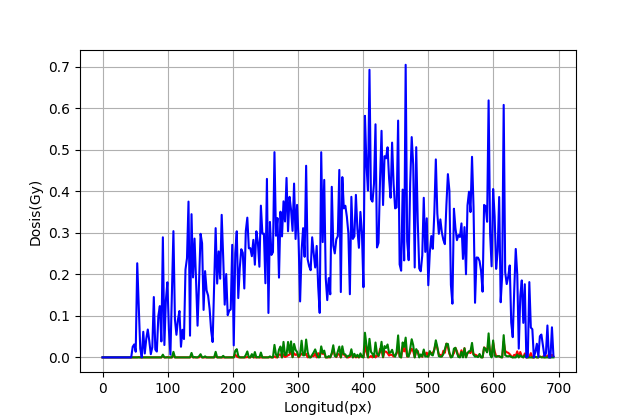
\includegraphics[width=.5\linewidth]{images/perfilDosisCeroVerticalEnCentro.png} 
		\caption{Perfil de dosis vertical} 
		\vspace{4ex}
	\end{minipage} 
\caption{Perfiles de dosis de película sin irradiar}
\label{fig:perfiles} 
\end{figure}

En estos perfiles se evidencia un sesgo sistemático en la dosis predicha para la película en cada punto. Se esperaría que, salvo variaciones muy pequeñas, los perfiles de dosis siempre dieran valores cercanos a cero. Sin embargo se observan varios comportamientos defectuosos reportados en la literatura. Se evidencia que en los tres canales de color se sobre-estima la dosis cuando el punto de estimación está lejos del eje central del escáner, es decir, cerca de los bordes.\\

También se evidencia que el canal azul proporciona medidas erradas de dosis por la poca sensibilidad que tiene la película en ese rango de dosis, lo que permite decir que no debe ser usado para otros objetivas más que la calibración multicanal.\\

Otra propiedad que permite evidenciar estos perfiles es la gran cantidad de ruido que mide el escáner, lo cual se ve las grandes variaciones locales en los perfiles de dosis. Esto es consecuencia de varios factores, el principal de ellos son los pixeles defectuosos que el escáner pueda tener. Para identificar estos pixeles defectuosos se cubrió el área de escaneo que se estaba usando con abundante cartulina negra, obteniendo la imagen escaneada que se muestra en la figura \ref{fig:fondoNegro}. En detalle se observan los pixeles absorben luz cuando no deberían. \\

\begin{figure}[H]
	\centering
	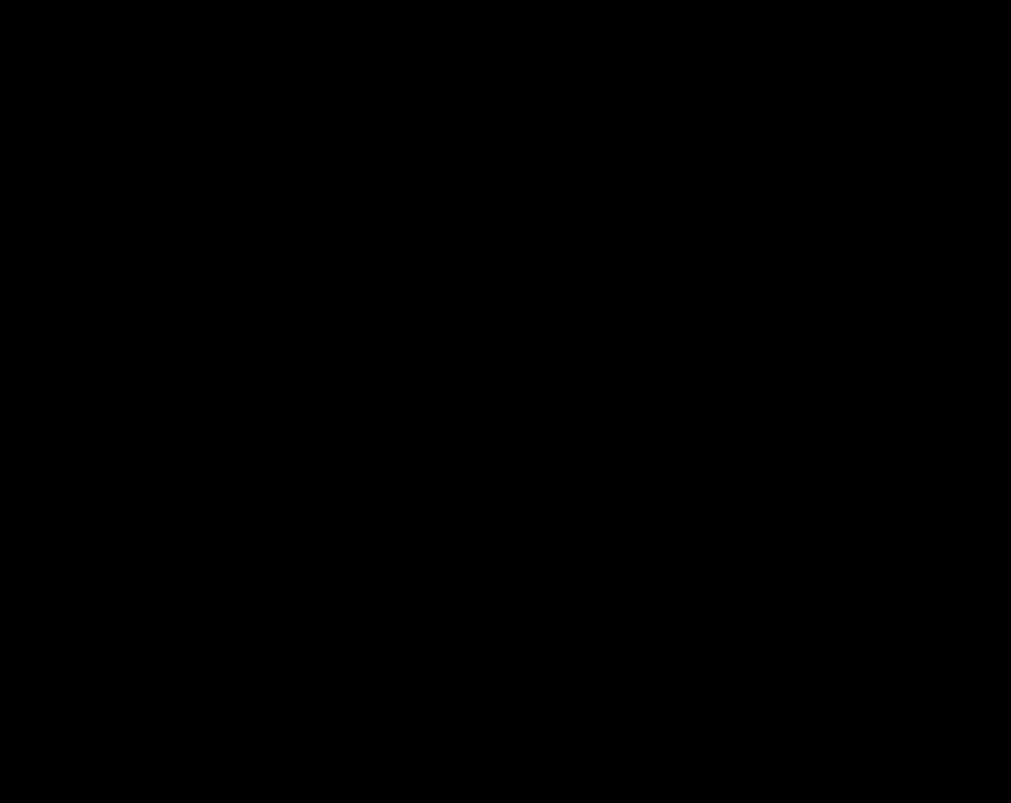
\includegraphics[width=0.7\linewidth]{images/FondoNegro.png}
	\caption{Pixeles defectuosos del escáner }
	\label{fig:fondoNegro}
\end{figure}

Para corregir parte de este ruido en las posteriores tomas se escaneo cada imagen múltiples veces, lo que reduce la cantidad de pixeles defectuosos.\\

Para continuar realizando pruebas en los métodos usados se analiza el cuadrado de 5 Gy de 10x10 cm que se irradió. La película resultante se muestra en la figura \ref{fig:cuadrado5Gy}. En este se muestran los puntos fiduciales que se usan para identificar el eje del campo.\\

\begin{figure}[H]
	\centering
	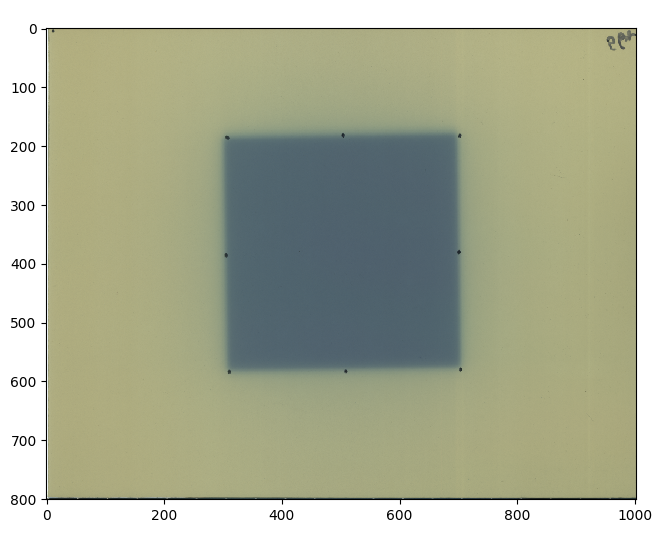
\includegraphics[width=0.7\linewidth]{images/peliculaCuadrado.png}
	\caption{Película irradiada con cuadrado de 5 Gy }
	\label{fig:cuadrado5Gy}
\end{figure}

Este cuadrado sirve para identificar fácilmente las ventajas del método multicanal con respecto a la calibración mediante canales individuales. En la figura \ref{fig:MapaCuadrado} se muestra el mapa de dosis del cuadrado obtenido junto con la sepración que este método realiza de las partes de la transmitancia que son independientes de la dosis que se absorbió.\\
\begin{figure}[H]
	\centering
	\subfloat[Mapa de dosis del cuadrado de 5 Gy]{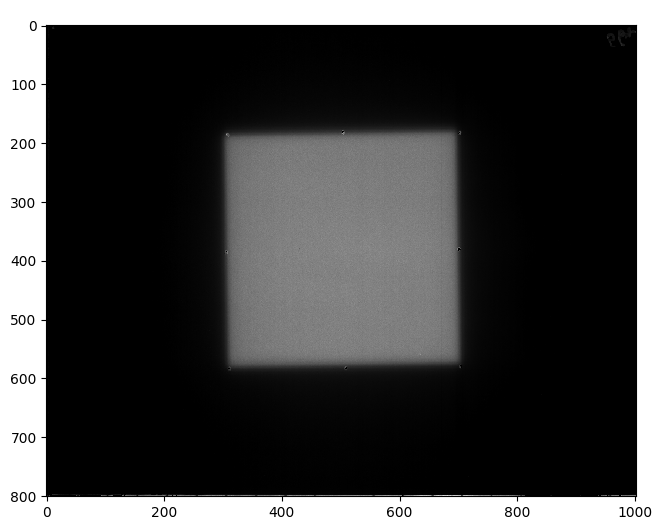
\includegraphics[width=0.5\textwidth]{images/mapaCuadradoConMulticanal.png}\label{fig:MapaCuadradoMulti}}
	\hfill
	\subfloat[Defectos de la película obtenidos con el método multicanal]{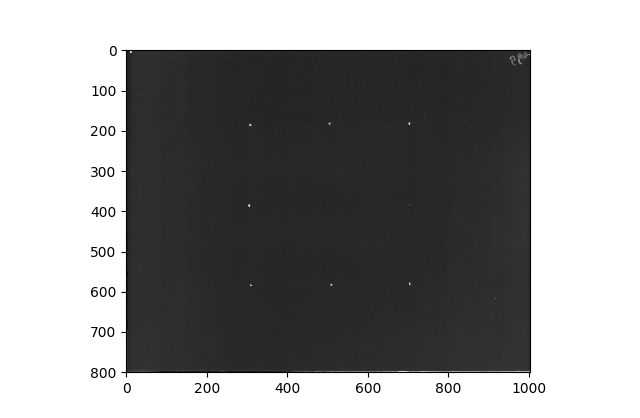
\includegraphics[width=0.8\textwidth]{images/imperfeccionesPeliculaCuadrado.png}\label{fig:fondoCuadrado5Gy}}
	\caption{Mapa de dosis obtenido con el método multicanal}
	\label{fig:MapaCuadrado}
\end{figure}

En el mapa de defectos se encuentran tanto los puntos fiduciales, como las barras transportadoras propias del escáner. Estas componentes ya no son tenidas en cuenta en el calculo de dosis de cada punto. Esto resulta finalmente en un mapa de dosis más limpio, libre de una gran parte de irregularidades y efectos asociados a inhomogeneidades de la película.\\

Podemos comparar los perfiles de dosis sobre una linea que pasa por centro de cuadrado obtenidos con canales individuales y usando el método multicanal. En la figura \ref{fig:perfilesMapaCuadrado} se muestran perfiles centrales obtenidos con cada método. Se observa cómo se reduce el rudio con el método multicanal, resultando en un medida fiable de la dosis obtenida en cada punto. 
\begin{figure}[H]
	\centering
	\subfloat[Perfil de dosis central con método de un solo canal]{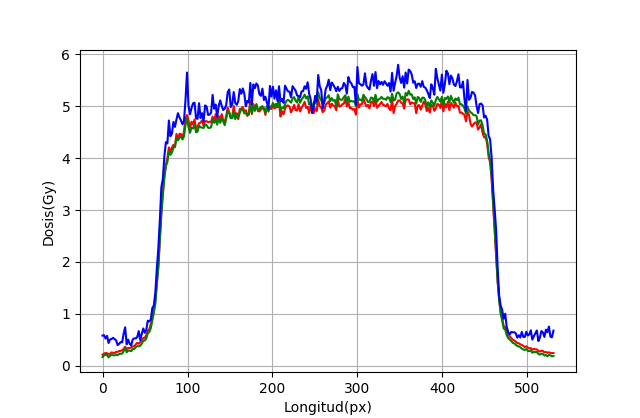
\includegraphics[width=0.7\textwidth]{images/perfilDosisCuadradoUnoSolo.png}\label{fig:perfilSolo}}
	\hfill
	\subfloat[Perfil de dosis central con método multicanal ]{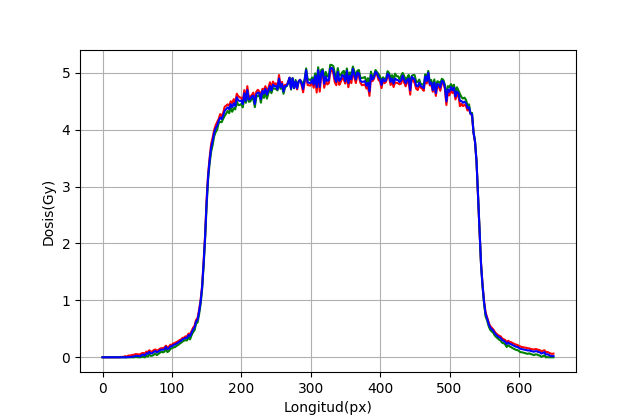
\includegraphics[width=0.7\textwidth]{images/perfilDosisCuadradoMulticanal.png}\label{fig:perfilMultiple}}
	\caption{Perfil central de dosis en película con cuadrado de 5 Gy}
	\label{fig:perfilesMapaCuadrado}
\end{figure}

Otra manera de observar la superioridad del método multicanal sobre el método de un solo canal es observar el mismo perfil, que se muestra en la figura \ref{fig:perfilCero}, sobre la película sin irradiar como en la figura \ref{fig:perhor} pero ahora en el mapa calculado con la calibración multicanal. Aquí se evidencia también que este método es útil para corregir la sobreestimación debida a la cercanía al borde del escáner.\\

\begin{figure}[H]
	\centering
	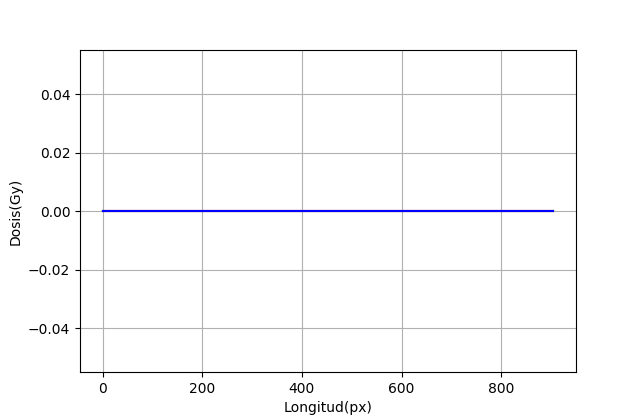
\includegraphics[width=0.7\linewidth]{images/perfilHorizontalDeDosisCeroMulticanal.png}
	\caption{Perfil de dosis horizontal en película sin irradiar con método multicanal }
	\label{fig:perfilCero}
\end{figure}

También se produjo la separación de las componentes independientes de dosis en la película sin irradiar, las cuales se muestran en la figura \ref{fig:irregularCero} 
\begin{figure}[H]
	\centering
	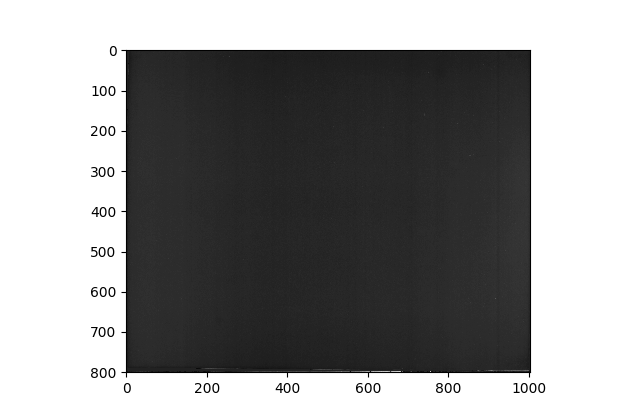
\includegraphics[width=0.7\linewidth]{images/fondoIndependienteDosisPeliculaCero.png}
	\caption{Irregularidades en película sin escanear obtenidas con método multicanal }
	\label{fig:irregularCero}
\end{figure}

Por otro lado, también se investigó la diferencia en ruido al usar canales de color de 8 o 16 bits. En la figura  \ref{fig:8o16} se muestran perfiles centrales para el cuadrado de 5 Gy cuando la película se escanea en modo de 8 y 16 bits. Aquí se evidencia que usando 8 bits se presentan mayores diferencias entre las dosis calculadas en cada canal debido a la menor capacidad de diferenciar colores. Se encontró que, contrario a lo que se esperaba, usar 8 bits de profundidad por canal de color presenta más ruido en la determinación de la dosis que usar canales de 16 bits.\\
\begin{figure}[H]
	\centering
	\subfloat[Perfil de dosis central con profundidad de 8 bits]{\includegraphics[width=0.7\textwidth]{images/perfilCuadradoMenosBit.png}\label{fig:perfil8}}
	\hfill
	\subfloat[Perfil de dosis central con profundidad de 16 bits ]{\includegraphics[width=0.7\textwidth]{images/perfilDosisCuadradoUnoSolo.png}\label{fig:perfil16}}
	\caption{Perfil central de dosis en película con cuadrado de 5 Gy a 8 y 16 bits de profundidad de color}
	\label{fig:8o16}
\end{figure}

Finalmente, se comprobó la dependencia de la transmitancia mediada en el escáner dependiendo de la orientación de la película con respecto a la lampara de escaneo, provocada por la polarización que ocurre en la medida. Este efecto se ve en las curvas de calibración presentadas en la figura \ref{fig:efectoOrientacion}, en las cuales se evidencia un desplazamiento en las transmitancias promedio cuando se rota la misma película 90 grados en la misma posición de escaneo.\\
\begin{figure}[H]
	\centering
	\subfloat[Curva de calibración con películas sin rotar]{\includegraphics[width=0.7\textwidth]{images/calibracion0-20-sinRotar.png}\label{fig:sinRotar}}
	\hfill
	\subfloat[Curvas de calibración con películas rotadas 90 grados ]{\includegraphics[width=0.7\textwidth]{images/calibracion0-20-Rotadas.png}\label{fig:perfil16}}
	\caption{Efecto de la orientación de escaneo sobre las transmitancias medidas}
	\label{fig:efectoOrientacion}
\end{figure}
Este efecto no es significativo en las medidas tomadas siempre y cuando se procuren orientar las películas cada vez en la misma dirección con respecto a la lampara del escáner.\\

No fue posible comprobar el efecto de otras variables como la temperatura y el tiempo post-exposición dadas las restricciones de tiempo y movilidad que se presentaron en el transcurso del trabajo, además de la poca capacidad de control que se tiene sobre estas variables en el transcurso del proceso.\\

\section{Mapas de dosis}


El plan piramidal de prueba produjo una película resultante que se ilustra en la figura \\
\begin{figure}
	\centering
	\missingfigure[figwidth=\linewidth,figcolor=white]{Plan de tratamiento}
	
	\caption{Pelicula EBT3 irradiada con plan de piramide }
	\label{fig:piramideEscaneada}
\end{figure}

En la figura \ref{fig:mapaPiramide} se muestra el mapa de dosis calculado con la digitalización anterior, junto al mapa de dosis que calculó el sistema de planeación en el mismo plano. Para alinear estos planes se usaron cuatro puntos fiduciales y un proceso de registro usando la librería SimpleITK de python.\\

\begin{figure}
	\centering
	\missingfigure[figwidth=\linewidth,figcolor=white]{Plan de tratamiento piramide comparada}
	
	\caption{Mapa de dosis calculado experimental y computacionalmente }
	\label{fig:mapaPiramide}
\end{figure}

Se pueden obtener diversas estadísticas para comparar estos planes, por ejemplo, en la figura \ref{fig:perfilesDosisPiramide} se muestran perfiles de dosis a diferentes niveles que muestran una concordancia entre las dosis calculadas de ambas maneras.\\
\begin{figure}
	\centering
	\missingfigure[figwidth=\linewidth,figcolor=white]{Plan de tratamiento piramide comparada}
	
	\caption{Perfiles de dosis en diferentes planos }
	\label{fig:perfilesDosisPiramide}
\end{figure}
Igualmente, en la figura \ref{fig:histogramasDosisPiramide} se muestran comparaciones de los histogramas de dosis obtenidos.\\
\begin{figure}
	\centering
	\missingfigure[figwidth=\linewidth,figcolor=white]{Plan de tratamiento piramide comparada histograma}
	
	\caption{Histogramas de dosis para plan pirámide }
	\label{fig:histogramasDosisPiramide}
\end{figure}

Finalmente, en la figura \ref{fig:isodosisPiramide}  se presentan curvas de isodosis de estos mapas.\\ 
\begin{figure}
	\centering
	\missingfigure[figwidth=\linewidth,figcolor=white]{Plan de tratamiento piramide comparada isodosis}
	
	\caption{Curvas de isodosis para plan pirámide }
	\label{fig:isodosisPiramide}
\end{figure}

Similarmente, se realiza un análisis comparativo del plan de tratamiento de mama 
\begin{figure}
	\centering
	\missingfigure[figwidth=\linewidth,figcolor=white]{Plan de tratamiento mama}
	
	\caption{Plan de tratamiento de mama escaneado }
	\label{fig:mamaEscaneada}
\end{figure}
\begin{figure}
	\centering
	\missingfigure[figwidth=\linewidth,figcolor=white]{Mapas de dosis mama}
	
	\caption{Mapa de dosis para plan de mama }
	\label{fig:mapaMama}
\end{figure}
\begin{figure}
	\centering
	\missingfigure[figwidth=\linewidth,figcolor=white]{Plan de tratamiento piramide comparada isodosis}
	
	\caption{Curvas de isodosis para plan pirámide }
	\label{fig:histogramaMama}
\end{figure}
\begin{figure}
	\centering
	\missingfigure[figwidth=\linewidth,figcolor=white]{Plan de tratamiento piramide comparada isodosis}
	
	\caption{Curvas de isodosis para plan pirámide }
	\label{fig:isodosisMama}
\end{figure}

\section{Comparaciones $\Gamma$}

En el caso del plan pirámide, se obtiene la matriz $\Gamma$ mostrada en la figura \ref{fig:gammaPiramide}, así como el histograma de $\Gamma$ que evalúa la correspondencia general de los pixeles en ambas distribuciones.\\
\begin{figure}
	\centering
	\missingfigure[figwidth=\linewidth,figcolor=white]{Gamma Piramide}
	\caption{Análisis $\Gamma$ para plan piramide }
	\label{fig:gammaPiramide}
\end{figure}

Finalmente, en el caso del plan de tratamiento se mama, se muestra el mismo análisis en la figura \ref{fig:gammaMama}
\begin{figure}
	\centering
	\missingfigure[figwidth=\linewidth,figcolor=white]{Gamma mama}
	\caption{Análisis $\Gamma$ para plan de tratamiento de mama}
	\label{fig:gammaMama}
\end{figure}







\chapter{Conclusiones}
En este trabajo se encontró que las películas radiocrómicas son un instrumento útil para la garantía de calidad de procedimientos en radioterapia. Esto, debido a que proporcionan un método sencillo para realizar dosimetría relativa, permitiendo comparar las distribuciones de dosis entregadas realmente en un procedimiento de radioterapia con la planeadas en un principio.\\

Se estudiaron diversos fenómenos que se producen al trabajar con este tipo de películas, relacionados tanto a la parte de escaneo como a la parte de tratamiento digital posterior. Con base en ello, se estableció una metodología de escaneo y tratamiento que permite minimizar errores y obtener mapas de dosis reales listos para su comparación con los mapas planeados.\\

Todo el trabajo realizado es reproducible mediante el programa computacional diseñado y propuesto en los objetivos del proyecto. Este proporciona una interfaz amigable para el uso de estas películas en un ambiente clínico. Este posee las funcionalidades necesarias para realizar un proceso de calibración, generación de mapas de dosis y comparaciones mapa-plan que se requieren para asegurar la calidad del tratamiento.\\

\begin{appendices}
	\chapter{Diagramas de flujo}
	En la figura \ref{fig:diagramacalibracion} se muestra un diagrama de flujo que resume el proceso de calibración que se desarrolla en el programa.\\
\begin{figure}[H]
	\centering
	\includegraphics[width=\linewidth]{images/daigramaFlujo.png}
	\caption{Diagrama de flujo para calibración }
	\label{fig:diagramacalibracion}
\end{figure}
Análogamente, en la figura \ref{fig:diagramaMapa} se muestra un diagrama de flujo del proceso de construcción de un mapa de dosis.\\
\begin{figure}[H]
	\centering
	\includegraphics[width=\linewidth]{images/daigramaMapaDosis2.png}
	\caption{Diagrama de flujo para generación de mapa de dosis }
	\label{fig:diagramaMapa}
\end{figure}
Finalmente, en la figura \ref{fig:diagramaComparacion} se muestra un diagrama del proceso de comparación entre un plan calculado por el sistema de planeación y un mapa de dosis obtenido mediante una película radiocrómica.
\begin{figure}[H]
	\centering
	\includegraphics[width=\linewidth]{diagramaComparacion.png}
	\caption{Diagrama de flujo para comparación plan-mapa }
	\label{fig:diagramaComparacion}
\end{figure}
	\chapter{Documentación del programa}
	El programa desarrollado para el análisis de películas radiocrómicas proporciona varias funcionalidades para el usuario. En la figura \ref{fig:ventanaPrincipal} se muestra la ventana principal del programa.\\
\begin{figure}[H]
	\centering
	\includegraphics[width=0.7\linewidth]{images/imagenesDocumentacion/ventanaPrincipal.png}
	\caption{Ventana principal }
	\label{fig:ventanaPrincipal}
\end{figure}

En el menú superior se encuentran categorizadas las diversas funcionalidades que se requieren para realizar un análisis con películas radiocrómicas. En la parte derecha se encuentra un árbol de archivos que permite navegar entre los archivos abiertos actualmente en el programa, además del espacio del panel de control, donde se van a ubicar los botones de control dependiendo de la función requerida.\\

El primer menú permite realizar la calibración bajo diferentes configuraciones, a partir de una serie de películas irradiadas con diferentes dosis escaneadas en un formato tiff. En la figura \ref{fig:menuCalibracion} se muestran las diferentes opciones de configuración a las cuales el usuario tiene acceso.\\
\begin{figure}[H]
	\centering
	\includegraphics[width=0.7\linewidth]{images/imagenesDocumentacion/menuCalibracion.png}
	\caption{Menú de calibración }
	\label{fig:menuCalibracion}
\end{figure}

Después de la elección de configuración, se procede a la ventana de selección de ROIs que se usarán en la calibración. Esta ventana se muestra en la imagen \ref{fig:menuEleccionDosis}.
\begin{figure}[H]
	\centering
	\includegraphics[width=0.7\linewidth]{images/imagenesDocumentacion/menuEleccionDosis.png}
	\caption{Ventana de selección de ROI }
	\label{fig:menuEleccionDosis}
\end{figure}
Pulsando el botón de calibrar se creará un archivo de calibración(con extensión .calibr) que contiene la información del ajuste realizado con los datos que se consignan en la tabla mediante la interacción con la interfaz. Cada vez que se presione el botón de Nuevo ROI se promediara en la imagen las transmitancias del área elegida y se consignará este valor en la tabla.\\

En el menú de generación de mapas de dosis, al que se accede seleccionando el botón en la barra menú superior y que se muestra en la figura \ref{fig:menuMapaDosis} se elije un archivo de calibración y una imagen de una película escaneada en formato tiff. Además se eligen las opciones de filtros y correcciones por background.\\
\begin{figure}[H]
	\centering
	\includegraphics[width=0.7\linewidth]{images/imagenesDocumentacion/menuEleccionDosis.png}
	\caption{Menú para elección de características mapa de dosis }
	\label{fig:menuMapaDosis}
\end{figure}

Después de seleccionados estos parámetros se abre una ventana donde se muestra la película seleccionada, teniendo la opción de seleccionar y remover puntos fiduciarios, así como elegir solo una sección de esta para analizar. Esta ventana se muestra en la figura \ref{fig:ventanaMapaDosis1}.\\
\begin{figure}[H]
	\centering
	\includegraphics[width=0.7\linewidth]{images/imagenesDocumentacion/ventanaMapaDosis.png}
	\caption{Primera ventana para generación de mapas de dosis }
	\label{fig:ventanaMapaDosis1}
\end{figure}

Una vez se presione el botón de generar mapa, se realizará la conversión del área de la imagen seleccionada al mapa de dosis mediante la información del archivo de calibración seleccionado. Este mapa creado se muestra en otra ventana, que se ilustra en la figura \ref{fig:ventanaMapaDosis2}, y provee diversas opciones para el análisis del mismo. Así, se puede realizar un análisis interactivo de perfiles de dosis, histogramas de dosis y curvas de isodosis. También, se puede cambiar el punto de normalización de los mapas eligiendo entre tres opciones posibles. Finalmente, el botón guardar mapa empaquetará este mapa en formato DICOM y lo guardará en el disco.\\

\begin{figure}[H]
	\centering
	\includegraphics[width=0.7\linewidth]{images/imagenesDocumentacion/ventanaMapaDosis2.png}
	\caption{Segunda ventana para generación de mapas de dosis }
	\label{fig:ventanaMapaDosis2}
\end{figure}

Por último, el menú de comparación a plan, al que se accede por la barra menú en la parte superior, muestra las opciones que se pueden modificar para realizar el análisis $\Gamma$. Este menú se muestra en la figura \ref{fig:menuComparacion}.

\begin{figure}[H]
	\centering
	\includegraphics[width=0.7\linewidth]{images/imagenesDocumentacion/menuComparacionAplan.png}
	\caption{Menú para elegir las propiedades de comparación }
	\label{fig:menuComparacion}
\end{figure}

Lo cual abre una ventana donde se superponen los planes calculados y escaneados, así como las diversas opciones de comparación, incluyendo el análisis $\Gamma$ que se puede realizar. Esta última ventana se muestra en la figura \ref{fig:ventanaComparacion}

\begin{figure}[H]
	\centering
	\includegraphics[width=0.7\linewidth]{images/imagenesDocumentacion/ventanaComparacioAPlan.png}
	\caption{Ventana con opciones de comparación }
	\label{fig:ventanaComparacion}
\end{figure}


\end{appendices}
\nocite{*}
\bibliography{references}
\bibliographystyle{IEEEtran}

\end{document}